\begin{titlingpage}


    % ---------------------------------------------------- %
    % Main Info on Contents                                %
    % ---------------------------------------------------- %
    \newcommand{\infotable}{%
        \begin{tabular}{r|l}
            \textsc{\textbf{Studiengang}}
            & Elektro- und Informationstechnik \\
            [4mm]

            \textsc{\textbf{Modul}}
            & Projekt 4 \\
            [4mm]

            \textsc{\textbf{Auftraggeber}}
            & Hans Gysin \\
            [4mm]

            \textsc{\textbf{Betreuer}}
            & Matthias Meier, Pascal Schleuniger, Pascal Buchschacher, \\
            & Anita Gertiser, Bonnie Domenghino \\
            [4mm]

            \textsc{\textbf{Team}}
            & 3 \\
            [4mm]

            \textsc{\textbf{Autor}}
            & Reto Nussbaumer \\
            [4mm]

            \textsc{\textbf{Datum}}
            & \today \\
            [4mm]

            \textsc{\textbf{Version}}
            & 1 \\
        \end{tabular}%
    }%


    % ---------------------------------------------------- %
    % Place the Background Picture and Info Table          %
    % ---------------------------------------------------- %
    \hspace{-2.54mm}
    \newlength{\logoX}
    \setlength{\logoX}{5mm}
    \newlength{\logoY}
    \setlength{\logoY}{5mm}
    \begin{tikzpicture}[remember picture, overlay]
        % ------------------------------------------------ %
        % Background Picture                               %
        % ------------------------------------------------ %
        \node[inner sep=0pt] at (current page.center) {%
            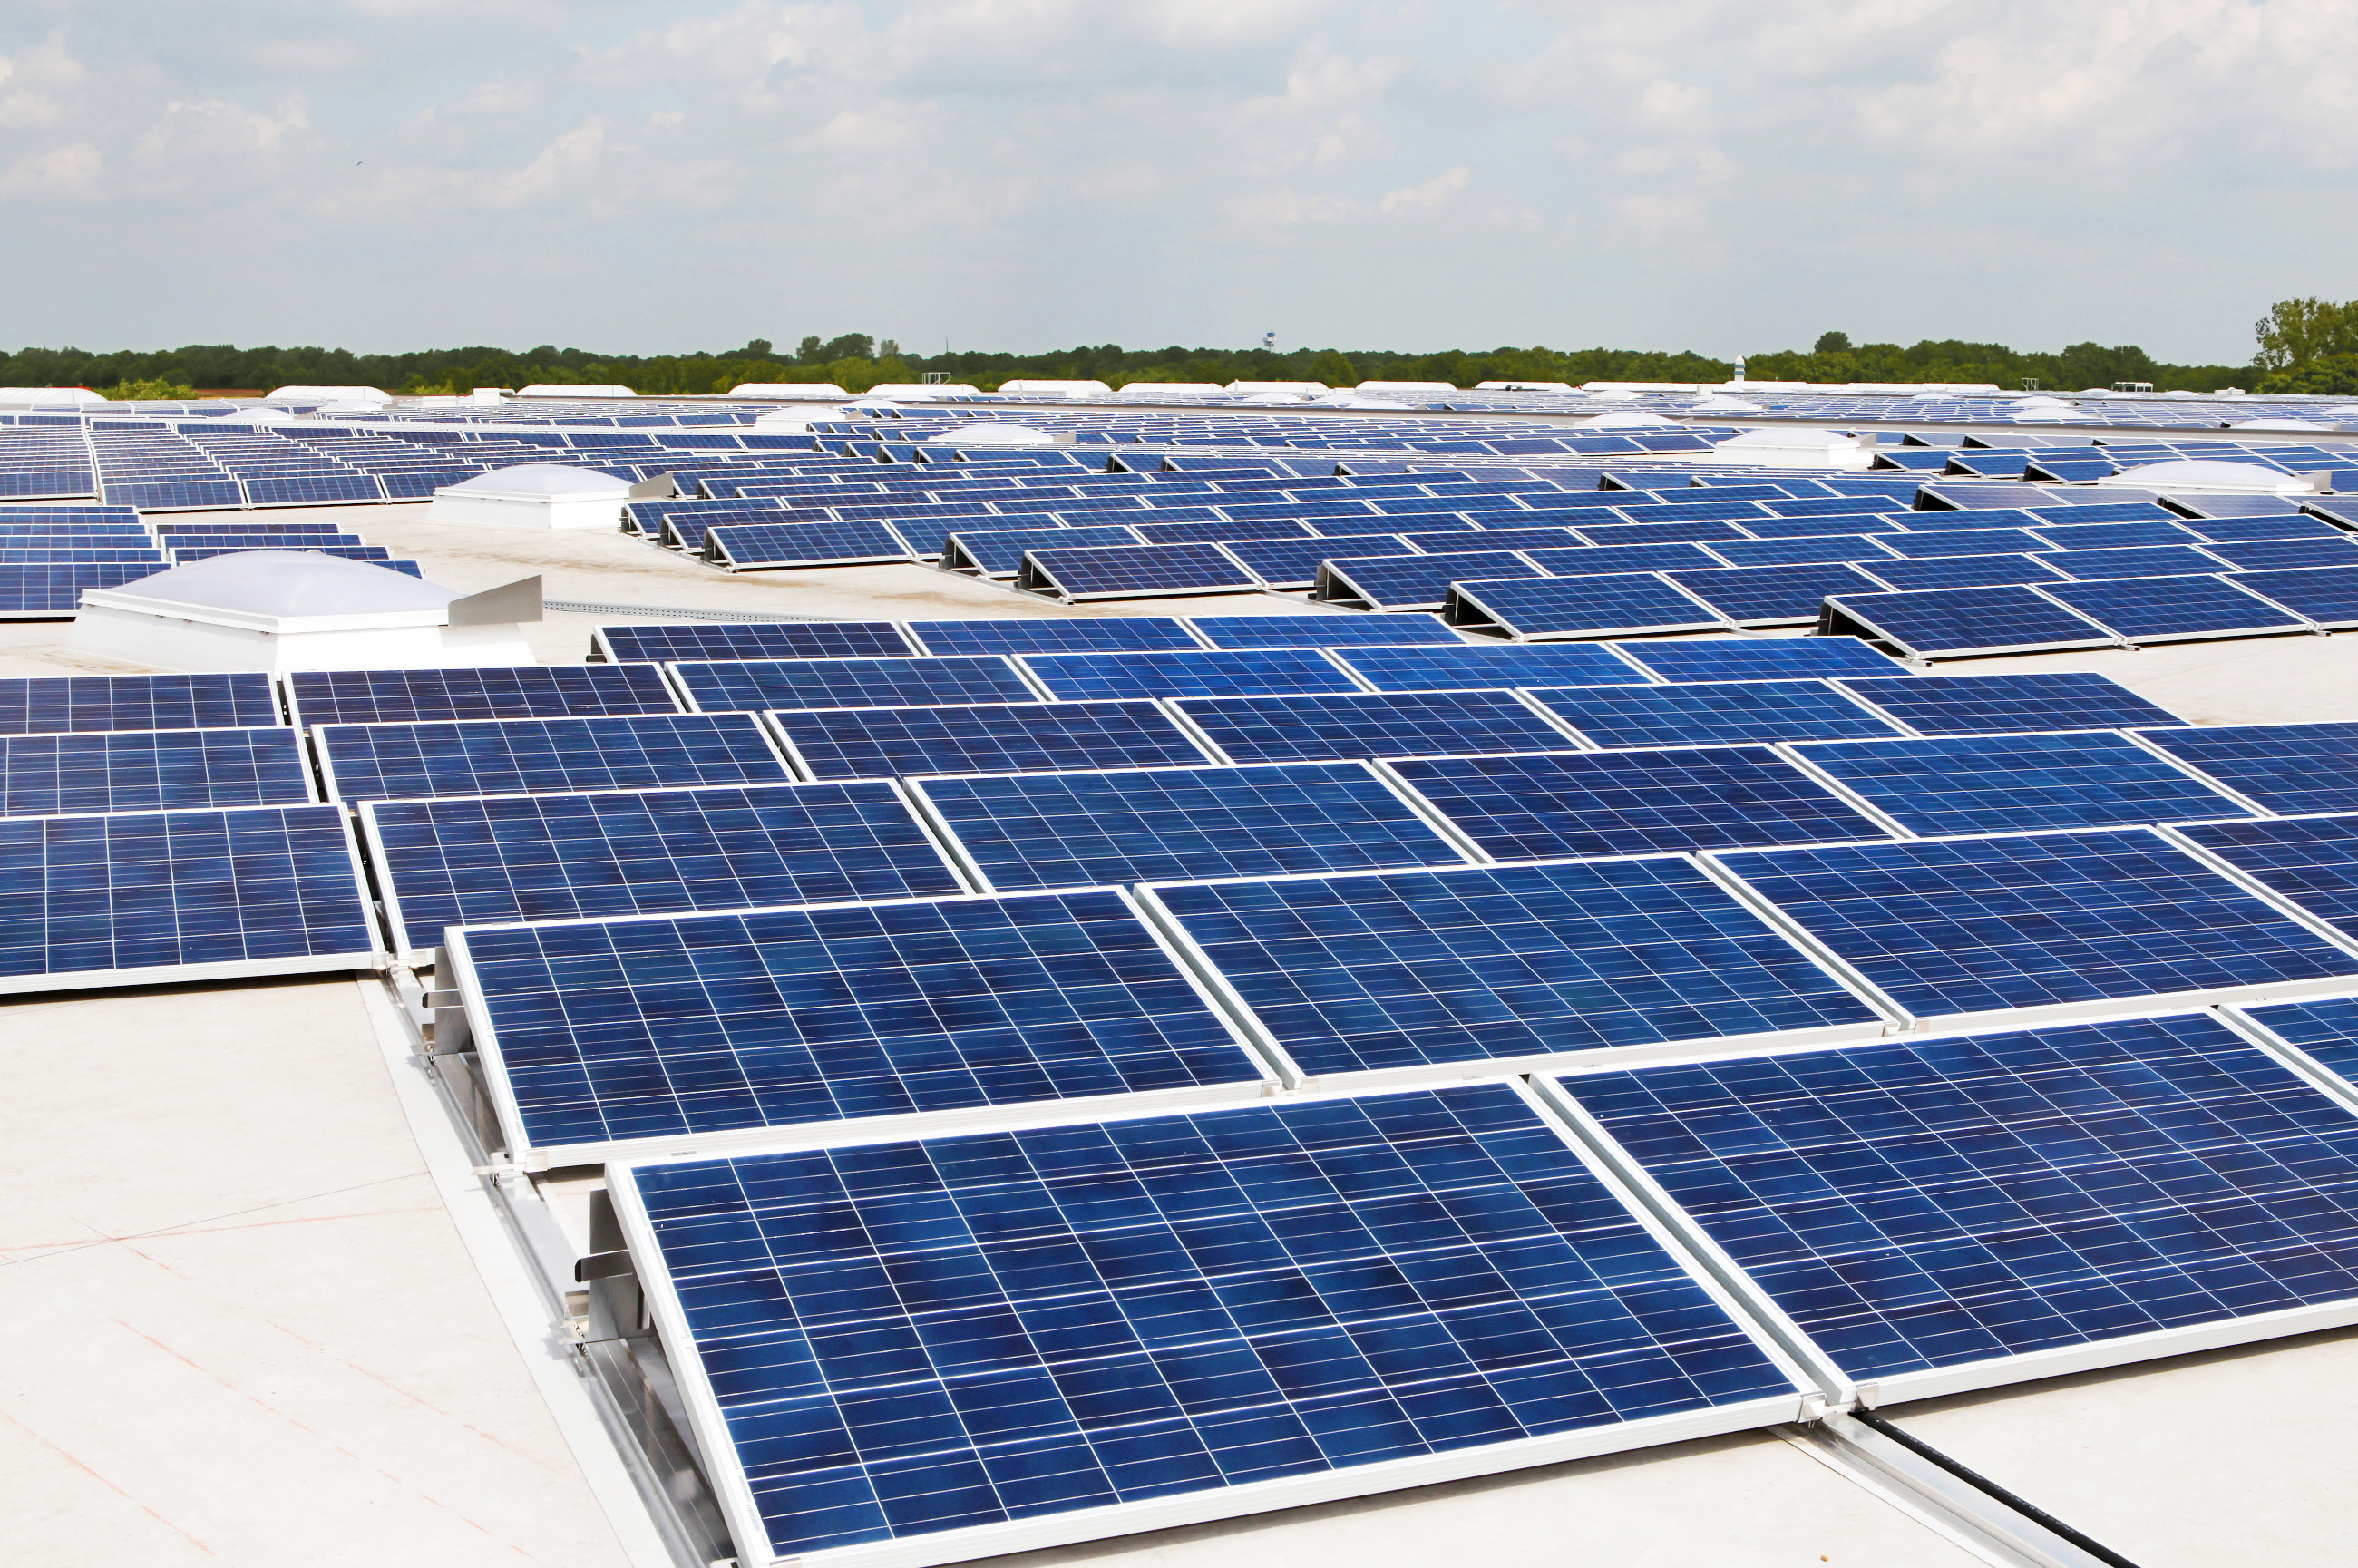
\includegraphics[width=\paperwidth,height=\paperheight]{images/titlepage/titlepic.jpg}%
        };
        %\node[
        %    fill=white,
        %    fill opacity=0.5,
        %    inner sep=0pt,
        %    anchor=west
        %] at (-38.5mm,-105mm) {%
        %    %% Creator: Matplotlib, PGF backend
%%
%% To include the figure in your LaTeX document, write
%%   \input{<filename>.pgf}
%%
%% Make sure the required packages are loaded in your preamble
%%   \usepackage{pgf}
%%
%% Figures using additional raster images can only be included by \input if
%% they are in the same directory as the main LaTeX file. For loading figures
%% from other directories you can use the `import` package
%%   \usepackage{import}
%% and then include the figures with
%%   \import{<path to file>}{<filename>.pgf}
%%
%% Matplotlib used the following preamble
%%   \usepackage{fontspec}
%%   \setmainfont{Bitstream Vera Serif}
%%   \setsansfont{Bitstream Vera Sans}
%%   \setmonofont{Bitstream Vera Sans Mono}
%%
\begingroup%
\makeatletter%
\begin{pgfpicture}%
\pgfpathrectangle{\pgfpointorigin}{\pgfqpoint{8.267700in}{2.000000in}}%
\pgfusepath{use as bounding box, clip}%
\begin{pgfscope}%
\pgfsetbuttcap%
\pgfsetmiterjoin%
\pgfsetlinewidth{0.000000pt}%
\definecolor{currentstroke}{rgb}{0.000000,0.000000,0.000000}%
\pgfsetstrokecolor{currentstroke}%
\pgfsetstrokeopacity{0.000000}%
\pgfsetdash{}{0pt}%
\pgfpathmoveto{\pgfqpoint{0.000000in}{0.000000in}}%
\pgfpathlineto{\pgfqpoint{8.267700in}{0.000000in}}%
\pgfpathlineto{\pgfqpoint{8.267700in}{2.000000in}}%
\pgfpathlineto{\pgfqpoint{0.000000in}{2.000000in}}%
\pgfpathclose%
\pgfusepath{}%
\end{pgfscope}%
\begin{pgfscope}%
\pgfsetbuttcap%
\pgfsetmiterjoin%
\pgfsetlinewidth{0.000000pt}%
\definecolor{currentstroke}{rgb}{0.000000,0.000000,0.000000}%
\pgfsetstrokecolor{currentstroke}%
\pgfsetstrokeopacity{0.000000}%
\pgfsetdash{}{0pt}%
\pgfpathmoveto{\pgfqpoint{0.000000in}{0.000000in}}%
\pgfpathlineto{\pgfqpoint{8.267700in}{0.000000in}}%
\pgfpathlineto{\pgfqpoint{8.267700in}{2.000000in}}%
\pgfpathlineto{\pgfqpoint{0.000000in}{2.000000in}}%
\pgfpathclose%
\pgfusepath{}%
\end{pgfscope}%
\begin{pgfscope}%
\pgfpathrectangle{\pgfqpoint{0.000000in}{0.000000in}}{\pgfqpoint{8.267700in}{2.000000in}} %
\pgfusepath{clip}%
\pgfsetrectcap%
\pgfsetroundjoin%
\pgfsetlinewidth{8.030000pt}%
\definecolor{currentstroke}{rgb}{1.000000,1.000000,1.000000}%
\pgfsetstrokecolor{currentstroke}%
\pgfsetdash{}{0pt}%
\pgfpathmoveto{\pgfqpoint{0.000000in}{1.000000in}}%
\pgfpathlineto{\pgfqpoint{0.044139in}{1.059355in}}%
\pgfpathlineto{\pgfqpoint{0.068966in}{1.089135in}}%
\pgfpathlineto{\pgfqpoint{0.088277in}{1.109222in}}%
\pgfpathlineto{\pgfqpoint{0.104829in}{1.123771in}}%
\pgfpathlineto{\pgfqpoint{0.121381in}{1.135506in}}%
\pgfpathlineto{\pgfqpoint{0.135174in}{1.142939in}}%
\pgfpathlineto{\pgfqpoint{0.148968in}{1.148114in}}%
\pgfpathlineto{\pgfqpoint{0.162761in}{1.150949in}}%
\pgfpathlineto{\pgfqpoint{0.176554in}{1.151398in}}%
\pgfpathlineto{\pgfqpoint{0.190347in}{1.149455in}}%
\pgfpathlineto{\pgfqpoint{0.204141in}{1.145150in}}%
\pgfpathlineto{\pgfqpoint{0.217934in}{1.138551in}}%
\pgfpathlineto{\pgfqpoint{0.234486in}{1.127755in}}%
\pgfpathlineto{\pgfqpoint{0.251038in}{1.114052in}}%
\pgfpathlineto{\pgfqpoint{0.270349in}{1.094814in}}%
\pgfpathlineto{\pgfqpoint{0.292418in}{1.069274in}}%
\pgfpathlineto{\pgfqpoint{0.320004in}{1.033549in}}%
\pgfpathlineto{\pgfqpoint{0.402764in}{0.923213in}}%
\pgfpathlineto{\pgfqpoint{0.424833in}{0.898652in}}%
\pgfpathlineto{\pgfqpoint{0.444144in}{0.880487in}}%
\pgfpathlineto{\pgfqpoint{0.460696in}{0.867841in}}%
\pgfpathlineto{\pgfqpoint{0.477248in}{0.858201in}}%
\pgfpathlineto{\pgfqpoint{0.491041in}{0.852624in}}%
\pgfpathlineto{\pgfqpoint{0.504835in}{0.849376in}}%
\pgfpathlineto{\pgfqpoint{0.518628in}{0.848508in}}%
\pgfpathlineto{\pgfqpoint{0.532421in}{0.850033in}}%
\pgfpathlineto{\pgfqpoint{0.546214in}{0.853929in}}%
\pgfpathlineto{\pgfqpoint{0.560008in}{0.860132in}}%
\pgfpathlineto{\pgfqpoint{0.573801in}{0.868546in}}%
\pgfpathlineto{\pgfqpoint{0.590353in}{0.881371in}}%
\pgfpathlineto{\pgfqpoint{0.606905in}{0.896894in}}%
\pgfpathlineto{\pgfqpoint{0.626216in}{0.917939in}}%
\pgfpathlineto{\pgfqpoint{0.651043in}{0.948627in}}%
\pgfpathlineto{\pgfqpoint{0.686906in}{0.997141in}}%
\pgfpathlineto{\pgfqpoint{0.733803in}{1.060231in}}%
\pgfpathlineto{\pgfqpoint{0.758631in}{1.089904in}}%
\pgfpathlineto{\pgfqpoint{0.777942in}{1.109881in}}%
\pgfpathlineto{\pgfqpoint{0.794494in}{1.124319in}}%
\pgfpathlineto{\pgfqpoint{0.811046in}{1.135929in}}%
\pgfpathlineto{\pgfqpoint{0.824839in}{1.143253in}}%
\pgfpathlineto{\pgfqpoint{0.838632in}{1.148312in}}%
\pgfpathlineto{\pgfqpoint{0.852426in}{1.151028in}}%
\pgfpathlineto{\pgfqpoint{0.866219in}{1.151358in}}%
\pgfpathlineto{\pgfqpoint{0.880012in}{1.149295in}}%
\pgfpathlineto{\pgfqpoint{0.893805in}{1.144874in}}%
\pgfpathlineto{\pgfqpoint{0.907599in}{1.138163in}}%
\pgfpathlineto{\pgfqpoint{0.924151in}{1.127240in}}%
\pgfpathlineto{\pgfqpoint{0.940703in}{1.113423in}}%
\pgfpathlineto{\pgfqpoint{0.960013in}{1.094068in}}%
\pgfpathlineto{\pgfqpoint{0.982082in}{1.068425in}}%
\pgfpathlineto{\pgfqpoint{1.009669in}{1.032619in}}%
\pgfpathlineto{\pgfqpoint{1.092429in}{0.922393in}}%
\pgfpathlineto{\pgfqpoint{1.114498in}{0.897946in}}%
\pgfpathlineto{\pgfqpoint{1.133809in}{0.879904in}}%
\pgfpathlineto{\pgfqpoint{1.150361in}{0.867378in}}%
\pgfpathlineto{\pgfqpoint{1.166913in}{0.857868in}}%
\pgfpathlineto{\pgfqpoint{1.180706in}{0.852406in}}%
\pgfpathlineto{\pgfqpoint{1.194499in}{0.849275in}}%
\pgfpathlineto{\pgfqpoint{1.208292in}{0.848527in}}%
\pgfpathlineto{\pgfqpoint{1.222086in}{0.850172in}}%
\pgfpathlineto{\pgfqpoint{1.235879in}{0.854185in}}%
\pgfpathlineto{\pgfqpoint{1.249672in}{0.860502in}}%
\pgfpathlineto{\pgfqpoint{1.263466in}{0.869023in}}%
\pgfpathlineto{\pgfqpoint{1.280018in}{0.881966in}}%
\pgfpathlineto{\pgfqpoint{1.299328in}{0.900435in}}%
\pgfpathlineto{\pgfqpoint{1.321397in}{0.925276in}}%
\pgfpathlineto{\pgfqpoint{1.346225in}{0.956773in}}%
\pgfpathlineto{\pgfqpoint{1.393123in}{1.020898in}}%
\pgfpathlineto{\pgfqpoint{1.426227in}{1.064572in}}%
\pgfpathlineto{\pgfqpoint{1.451054in}{1.093694in}}%
\pgfpathlineto{\pgfqpoint{1.470365in}{1.113106in}}%
\pgfpathlineto{\pgfqpoint{1.486917in}{1.126980in}}%
\pgfpathlineto{\pgfqpoint{1.503469in}{1.137967in}}%
\pgfpathlineto{\pgfqpoint{1.517262in}{1.144734in}}%
\pgfpathlineto{\pgfqpoint{1.531056in}{1.149213in}}%
\pgfpathlineto{\pgfqpoint{1.544849in}{1.151335in}}%
\pgfpathlineto{\pgfqpoint{1.558642in}{1.151066in}}%
\pgfpathlineto{\pgfqpoint{1.572435in}{1.148409in}}%
\pgfpathlineto{\pgfqpoint{1.586229in}{1.143407in}}%
\pgfpathlineto{\pgfqpoint{1.600022in}{1.136139in}}%
\pgfpathlineto{\pgfqpoint{1.616574in}{1.124590in}}%
\pgfpathlineto{\pgfqpoint{1.633126in}{1.110208in}}%
\pgfpathlineto{\pgfqpoint{1.652437in}{1.090287in}}%
\pgfpathlineto{\pgfqpoint{1.674506in}{1.064141in}}%
\pgfpathlineto{\pgfqpoint{1.704851in}{1.024196in}}%
\pgfpathlineto{\pgfqpoint{1.773818in}{0.931575in}}%
\pgfpathlineto{\pgfqpoint{1.795887in}{0.905932in}}%
\pgfpathlineto{\pgfqpoint{1.815197in}{0.886577in}}%
\pgfpathlineto{\pgfqpoint{1.831749in}{0.872760in}}%
\pgfpathlineto{\pgfqpoint{1.848301in}{0.861837in}}%
\pgfpathlineto{\pgfqpoint{1.862095in}{0.855126in}}%
\pgfpathlineto{\pgfqpoint{1.875888in}{0.850705in}}%
\pgfpathlineto{\pgfqpoint{1.889681in}{0.848642in}}%
\pgfpathlineto{\pgfqpoint{1.903474in}{0.848972in}}%
\pgfpathlineto{\pgfqpoint{1.917268in}{0.851688in}}%
\pgfpathlineto{\pgfqpoint{1.931061in}{0.856747in}}%
\pgfpathlineto{\pgfqpoint{1.944854in}{0.864071in}}%
\pgfpathlineto{\pgfqpoint{1.961406in}{0.875681in}}%
\pgfpathlineto{\pgfqpoint{1.977958in}{0.890119in}}%
\pgfpathlineto{\pgfqpoint{1.997269in}{0.910096in}}%
\pgfpathlineto{\pgfqpoint{2.019338in}{0.936291in}}%
\pgfpathlineto{\pgfqpoint{2.049683in}{0.976274in}}%
\pgfpathlineto{\pgfqpoint{2.118650in}{1.068850in}}%
\pgfpathlineto{\pgfqpoint{2.140719in}{1.094442in}}%
\pgfpathlineto{\pgfqpoint{2.160030in}{1.113738in}}%
\pgfpathlineto{\pgfqpoint{2.176582in}{1.127498in}}%
\pgfpathlineto{\pgfqpoint{2.193134in}{1.138358in}}%
\pgfpathlineto{\pgfqpoint{2.206927in}{1.145013in}}%
\pgfpathlineto{\pgfqpoint{2.220720in}{1.149376in}}%
\pgfpathlineto{\pgfqpoint{2.234514in}{1.151379in}}%
\pgfpathlineto{\pgfqpoint{2.248307in}{1.150989in}}%
\pgfpathlineto{\pgfqpoint{2.262100in}{1.148214in}}%
\pgfpathlineto{\pgfqpoint{2.275893in}{1.143097in}}%
\pgfpathlineto{\pgfqpoint{2.289687in}{1.135718in}}%
\pgfpathlineto{\pgfqpoint{2.306239in}{1.124046in}}%
\pgfpathlineto{\pgfqpoint{2.322791in}{1.109552in}}%
\pgfpathlineto{\pgfqpoint{2.342101in}{1.089520in}}%
\pgfpathlineto{\pgfqpoint{2.364170in}{1.063276in}}%
\pgfpathlineto{\pgfqpoint{2.394516in}{1.023255in}}%
\pgfpathlineto{\pgfqpoint{2.463482in}{0.930726in}}%
\pgfpathlineto{\pgfqpoint{2.485551in}{0.905186in}}%
\pgfpathlineto{\pgfqpoint{2.504862in}{0.885948in}}%
\pgfpathlineto{\pgfqpoint{2.521414in}{0.872245in}}%
\pgfpathlineto{\pgfqpoint{2.537966in}{0.861449in}}%
\pgfpathlineto{\pgfqpoint{2.551759in}{0.854850in}}%
\pgfpathlineto{\pgfqpoint{2.565553in}{0.850545in}}%
\pgfpathlineto{\pgfqpoint{2.579346in}{0.848602in}}%
\pgfpathlineto{\pgfqpoint{2.593139in}{0.849051in}}%
\pgfpathlineto{\pgfqpoint{2.606932in}{0.851886in}}%
\pgfpathlineto{\pgfqpoint{2.620726in}{0.857061in}}%
\pgfpathlineto{\pgfqpoint{2.634519in}{0.864494in}}%
\pgfpathlineto{\pgfqpoint{2.651071in}{0.876229in}}%
\pgfpathlineto{\pgfqpoint{2.667623in}{0.890778in}}%
\pgfpathlineto{\pgfqpoint{2.686934in}{0.910865in}}%
\pgfpathlineto{\pgfqpoint{2.709003in}{0.937157in}}%
\pgfpathlineto{\pgfqpoint{2.739348in}{0.977216in}}%
\pgfpathlineto{\pgfqpoint{2.755900in}{1.000000in}}%
\pgfpathlineto{\pgfqpoint{2.755900in}{1.000000in}}%
\pgfusepath{stroke}%
\end{pgfscope}%
\begin{pgfscope}%
\pgfpathrectangle{\pgfqpoint{0.000000in}{0.000000in}}{\pgfqpoint{8.267700in}{2.000000in}} %
\pgfusepath{clip}%
\pgfsetrectcap%
\pgfsetroundjoin%
\pgfsetlinewidth{8.030000pt}%
\definecolor{currentstroke}{rgb}{1.000000,1.000000,1.000000}%
\pgfsetstrokecolor{currentstroke}%
\pgfsetdash{}{0pt}%
\pgfpathmoveto{\pgfqpoint{2.755900in}{1.000000in}}%
\pgfpathlineto{\pgfqpoint{2.797280in}{1.334978in}}%
\pgfpathlineto{\pgfqpoint{2.819349in}{1.497163in}}%
\pgfpathlineto{\pgfqpoint{2.838660in}{1.622816in}}%
\pgfpathlineto{\pgfqpoint{2.855212in}{1.715316in}}%
\pgfpathlineto{\pgfqpoint{2.869005in}{1.780052in}}%
\pgfpathlineto{\pgfqpoint{2.880040in}{1.823008in}}%
\pgfpathlineto{\pgfqpoint{2.891074in}{1.857636in}}%
\pgfpathlineto{\pgfqpoint{2.899350in}{1.877929in}}%
\pgfpathlineto{\pgfqpoint{2.907626in}{1.893223in}}%
\pgfpathlineto{\pgfqpoint{2.915902in}{1.903432in}}%
\pgfpathlineto{\pgfqpoint{2.921420in}{1.907382in}}%
\pgfpathlineto{\pgfqpoint{2.926937in}{1.909036in}}%
\pgfpathlineto{\pgfqpoint{2.932454in}{1.908389in}}%
\pgfpathlineto{\pgfqpoint{2.937971in}{1.905442in}}%
\pgfpathlineto{\pgfqpoint{2.943489in}{1.900204in}}%
\pgfpathlineto{\pgfqpoint{2.951765in}{1.888080in}}%
\pgfpathlineto{\pgfqpoint{2.960041in}{1.870900in}}%
\pgfpathlineto{\pgfqpoint{2.968317in}{1.848761in}}%
\pgfpathlineto{\pgfqpoint{2.979351in}{1.811751in}}%
\pgfpathlineto{\pgfqpoint{2.990386in}{1.766527in}}%
\pgfpathlineto{\pgfqpoint{3.004179in}{1.699153in}}%
\pgfpathlineto{\pgfqpoint{3.017973in}{1.620730in}}%
\pgfpathlineto{\pgfqpoint{3.034525in}{1.513795in}}%
\pgfpathlineto{\pgfqpoint{3.053835in}{1.374456in}}%
\pgfpathlineto{\pgfqpoint{3.081422in}{1.156454in}}%
\pgfpathlineto{\pgfqpoint{3.150388in}{0.599683in}}%
\pgfpathlineto{\pgfqpoint{3.172457in}{0.444598in}}%
\pgfpathlineto{\pgfqpoint{3.189009in}{0.342688in}}%
\pgfpathlineto{\pgfqpoint{3.202803in}{0.269094in}}%
\pgfpathlineto{\pgfqpoint{3.216596in}{0.207049in}}%
\pgfpathlineto{\pgfqpoint{3.227631in}{0.166395in}}%
\pgfpathlineto{\pgfqpoint{3.238665in}{0.134175in}}%
\pgfpathlineto{\pgfqpoint{3.246941in}{0.115744in}}%
\pgfpathlineto{\pgfqpoint{3.255217in}{0.102349in}}%
\pgfpathlineto{\pgfqpoint{3.263493in}{0.094064in}}%
\pgfpathlineto{\pgfqpoint{3.269011in}{0.091405in}}%
\pgfpathlineto{\pgfqpoint{3.274528in}{0.091045in}}%
\pgfpathlineto{\pgfqpoint{3.280045in}{0.092986in}}%
\pgfpathlineto{\pgfqpoint{3.285562in}{0.097223in}}%
\pgfpathlineto{\pgfqpoint{3.291080in}{0.103745in}}%
\pgfpathlineto{\pgfqpoint{3.299356in}{0.117775in}}%
\pgfpathlineto{\pgfqpoint{3.307632in}{0.136828in}}%
\pgfpathlineto{\pgfqpoint{3.315908in}{0.160795in}}%
\pgfpathlineto{\pgfqpoint{3.326942in}{0.200156in}}%
\pgfpathlineto{\pgfqpoint{3.337977in}{0.247611in}}%
\pgfpathlineto{\pgfqpoint{3.351770in}{0.317571in}}%
\pgfpathlineto{\pgfqpoint{3.368322in}{0.415648in}}%
\pgfpathlineto{\pgfqpoint{3.387633in}{0.546693in}}%
\pgfpathlineto{\pgfqpoint{3.409702in}{0.713372in}}%
\pgfpathlineto{\pgfqpoint{3.442806in}{0.982848in}}%
\pgfpathlineto{\pgfqpoint{3.486945in}{1.340286in}}%
\pgfpathlineto{\pgfqpoint{3.509014in}{1.501940in}}%
\pgfpathlineto{\pgfqpoint{3.528324in}{1.626968in}}%
\pgfpathlineto{\pgfqpoint{3.544876in}{1.718831in}}%
\pgfpathlineto{\pgfqpoint{3.558670in}{1.782973in}}%
\pgfpathlineto{\pgfqpoint{3.569704in}{1.825420in}}%
\pgfpathlineto{\pgfqpoint{3.580739in}{1.859516in}}%
\pgfpathlineto{\pgfqpoint{3.589015in}{1.879396in}}%
\pgfpathlineto{\pgfqpoint{3.597291in}{1.894269in}}%
\pgfpathlineto{\pgfqpoint{3.605567in}{1.904051in}}%
\pgfpathlineto{\pgfqpoint{3.611084in}{1.907715in}}%
\pgfpathlineto{\pgfqpoint{3.616602in}{1.909081in}}%
\pgfpathlineto{\pgfqpoint{3.622119in}{1.908146in}}%
\pgfpathlineto{\pgfqpoint{3.627636in}{1.904912in}}%
\pgfpathlineto{\pgfqpoint{3.633153in}{1.899389in}}%
\pgfpathlineto{\pgfqpoint{3.641429in}{1.886840in}}%
\pgfpathlineto{\pgfqpoint{3.649705in}{1.869242in}}%
\pgfpathlineto{\pgfqpoint{3.657981in}{1.846696in}}%
\pgfpathlineto{\pgfqpoint{3.669016in}{1.809161in}}%
\pgfpathlineto{\pgfqpoint{3.680051in}{1.763438in}}%
\pgfpathlineto{\pgfqpoint{3.693844in}{1.695484in}}%
\pgfpathlineto{\pgfqpoint{3.707637in}{1.616540in}}%
\pgfpathlineto{\pgfqpoint{3.724189in}{1.509068in}}%
\pgfpathlineto{\pgfqpoint{3.743500in}{1.369238in}}%
\pgfpathlineto{\pgfqpoint{3.771086in}{1.150819in}}%
\pgfpathlineto{\pgfqpoint{3.840053in}{0.594558in}}%
\pgfpathlineto{\pgfqpoint{3.862122in}{0.440082in}}%
\pgfpathlineto{\pgfqpoint{3.878674in}{0.338751in}}%
\pgfpathlineto{\pgfqpoint{3.892467in}{0.265708in}}%
\pgfpathlineto{\pgfqpoint{3.906261in}{0.204268in}}%
\pgfpathlineto{\pgfqpoint{3.917295in}{0.164130in}}%
\pgfpathlineto{\pgfqpoint{3.928330in}{0.132449in}}%
\pgfpathlineto{\pgfqpoint{3.936606in}{0.114435in}}%
\pgfpathlineto{\pgfqpoint{3.944882in}{0.101462in}}%
\pgfpathlineto{\pgfqpoint{3.950399in}{0.095653in}}%
\pgfpathlineto{\pgfqpoint{3.955917in}{0.092133in}}%
\pgfpathlineto{\pgfqpoint{3.961434in}{0.090910in}}%
\pgfpathlineto{\pgfqpoint{3.966951in}{0.091989in}}%
\pgfpathlineto{\pgfqpoint{3.972468in}{0.095366in}}%
\pgfpathlineto{\pgfqpoint{3.977986in}{0.101032in}}%
\pgfpathlineto{\pgfqpoint{3.986262in}{0.113793in}}%
\pgfpathlineto{\pgfqpoint{3.994538in}{0.131599in}}%
\pgfpathlineto{\pgfqpoint{4.002814in}{0.154349in}}%
\pgfpathlineto{\pgfqpoint{4.013848in}{0.192146in}}%
\pgfpathlineto{\pgfqpoint{4.024883in}{0.238118in}}%
\pgfpathlineto{\pgfqpoint{4.038676in}{0.306360in}}%
\pgfpathlineto{\pgfqpoint{4.052470in}{0.385564in}}%
\pgfpathlineto{\pgfqpoint{4.069022in}{0.493303in}}%
\pgfpathlineto{\pgfqpoint{4.088332in}{0.633376in}}%
\pgfpathlineto{\pgfqpoint{4.115919in}{0.852001in}}%
\pgfpathlineto{\pgfqpoint{4.182127in}{1.387434in}}%
\pgfpathlineto{\pgfqpoint{4.204196in}{1.544017in}}%
\pgfpathlineto{\pgfqpoint{4.220748in}{1.647357in}}%
\pgfpathlineto{\pgfqpoint{4.234541in}{1.722317in}}%
\pgfpathlineto{\pgfqpoint{4.248334in}{1.785863in}}%
\pgfpathlineto{\pgfqpoint{4.259369in}{1.827800in}}%
\pgfpathlineto{\pgfqpoint{4.270404in}{1.861361in}}%
\pgfpathlineto{\pgfqpoint{4.278680in}{1.880828in}}%
\pgfpathlineto{\pgfqpoint{4.286956in}{1.895280in}}%
\pgfpathlineto{\pgfqpoint{4.295232in}{1.904634in}}%
\pgfpathlineto{\pgfqpoint{4.300749in}{1.908011in}}%
\pgfpathlineto{\pgfqpoint{4.306266in}{1.909090in}}%
\pgfpathlineto{\pgfqpoint{4.311783in}{1.907867in}}%
\pgfpathlineto{\pgfqpoint{4.317301in}{1.904347in}}%
\pgfpathlineto{\pgfqpoint{4.322818in}{1.898538in}}%
\pgfpathlineto{\pgfqpoint{4.331094in}{1.885565in}}%
\pgfpathlineto{\pgfqpoint{4.339370in}{1.867551in}}%
\pgfpathlineto{\pgfqpoint{4.347646in}{1.844597in}}%
\pgfpathlineto{\pgfqpoint{4.358681in}{1.806538in}}%
\pgfpathlineto{\pgfqpoint{4.369715in}{1.760319in}}%
\pgfpathlineto{\pgfqpoint{4.383509in}{1.691788in}}%
\pgfpathlineto{\pgfqpoint{4.397302in}{1.612326in}}%
\pgfpathlineto{\pgfqpoint{4.413854in}{1.504321in}}%
\pgfpathlineto{\pgfqpoint{4.433164in}{1.364006in}}%
\pgfpathlineto{\pgfqpoint{4.460751in}{1.145177in}}%
\pgfpathlineto{\pgfqpoint{4.526959in}{0.609981in}}%
\pgfpathlineto{\pgfqpoint{4.549028in}{0.453695in}}%
\pgfpathlineto{\pgfqpoint{4.565580in}{0.350639in}}%
\pgfpathlineto{\pgfqpoint{4.579373in}{0.275951in}}%
\pgfpathlineto{\pgfqpoint{4.593167in}{0.212704in}}%
\pgfpathlineto{\pgfqpoint{4.604201in}{0.171023in}}%
\pgfpathlineto{\pgfqpoint{4.615236in}{0.137729in}}%
\pgfpathlineto{\pgfqpoint{4.623512in}{0.118469in}}%
\pgfpathlineto{\pgfqpoint{4.631788in}{0.104228in}}%
\pgfpathlineto{\pgfqpoint{4.640064in}{0.095088in}}%
\pgfpathlineto{\pgfqpoint{4.645581in}{0.091854in}}%
\pgfpathlineto{\pgfqpoint{4.651098in}{0.090919in}}%
\pgfpathlineto{\pgfqpoint{4.656616in}{0.092285in}}%
\pgfpathlineto{\pgfqpoint{4.662133in}{0.095949in}}%
\pgfpathlineto{\pgfqpoint{4.667650in}{0.101901in}}%
\pgfpathlineto{\pgfqpoint{4.675926in}{0.115085in}}%
\pgfpathlineto{\pgfqpoint{4.684202in}{0.133308in}}%
\pgfpathlineto{\pgfqpoint{4.692478in}{0.156465in}}%
\pgfpathlineto{\pgfqpoint{4.703513in}{0.194785in}}%
\pgfpathlineto{\pgfqpoint{4.714548in}{0.241252in}}%
\pgfpathlineto{\pgfqpoint{4.728341in}{0.310070in}}%
\pgfpathlineto{\pgfqpoint{4.742134in}{0.389790in}}%
\pgfpathlineto{\pgfqpoint{4.758686in}{0.498060in}}%
\pgfpathlineto{\pgfqpoint{4.777997in}{0.638615in}}%
\pgfpathlineto{\pgfqpoint{4.805583in}{0.857646in}}%
\pgfpathlineto{\pgfqpoint{4.871791in}{1.392599in}}%
\pgfpathlineto{\pgfqpoint{4.893860in}{1.548587in}}%
\pgfpathlineto{\pgfqpoint{4.910412in}{1.651358in}}%
\pgfpathlineto{\pgfqpoint{4.924206in}{1.725774in}}%
\pgfpathlineto{\pgfqpoint{4.937999in}{1.788721in}}%
\pgfpathlineto{\pgfqpoint{4.949034in}{1.830147in}}%
\pgfpathlineto{\pgfqpoint{4.960068in}{1.863172in}}%
\pgfpathlineto{\pgfqpoint{4.968344in}{1.882225in}}%
\pgfpathlineto{\pgfqpoint{4.976620in}{1.896255in}}%
\pgfpathlineto{\pgfqpoint{4.984896in}{1.905182in}}%
\pgfpathlineto{\pgfqpoint{4.990414in}{1.908272in}}%
\pgfpathlineto{\pgfqpoint{4.995931in}{1.909063in}}%
\pgfpathlineto{\pgfqpoint{5.001448in}{1.907553in}}%
\pgfpathlineto{\pgfqpoint{5.006965in}{1.903746in}}%
\pgfpathlineto{\pgfqpoint{5.012483in}{1.897651in}}%
\pgfpathlineto{\pgfqpoint{5.020759in}{1.884256in}}%
\pgfpathlineto{\pgfqpoint{5.029035in}{1.865825in}}%
\pgfpathlineto{\pgfqpoint{5.037311in}{1.842465in}}%
\pgfpathlineto{\pgfqpoint{5.048345in}{1.803884in}}%
\pgfpathlineto{\pgfqpoint{5.059380in}{1.757169in}}%
\pgfpathlineto{\pgfqpoint{5.073173in}{1.688065in}}%
\pgfpathlineto{\pgfqpoint{5.089725in}{1.590896in}}%
\pgfpathlineto{\pgfqpoint{5.106277in}{1.480289in}}%
\pgfpathlineto{\pgfqpoint{5.128346in}{1.316294in}}%
\pgfpathlineto{\pgfqpoint{5.158692in}{1.071398in}}%
\pgfpathlineto{\pgfqpoint{5.211106in}{0.646501in}}%
\pgfpathlineto{\pgfqpoint{5.233175in}{0.486205in}}%
\pgfpathlineto{\pgfqpoint{5.252486in}{0.362759in}}%
\pgfpathlineto{\pgfqpoint{5.269038in}{0.272508in}}%
\pgfpathlineto{\pgfqpoint{5.282831in}{0.209861in}}%
\pgfpathlineto{\pgfqpoint{5.293866in}{0.168692in}}%
\pgfpathlineto{\pgfqpoint{5.304901in}{0.135935in}}%
\pgfpathlineto{\pgfqpoint{5.313177in}{0.117089in}}%
\pgfpathlineto{\pgfqpoint{5.321453in}{0.103271in}}%
\pgfpathlineto{\pgfqpoint{5.329729in}{0.094558in}}%
\pgfpathlineto{\pgfqpoint{5.335246in}{0.091611in}}%
\pgfpathlineto{\pgfqpoint{5.340763in}{0.090964in}}%
\pgfpathlineto{\pgfqpoint{5.346280in}{0.092618in}}%
\pgfpathlineto{\pgfqpoint{5.351798in}{0.096568in}}%
\pgfpathlineto{\pgfqpoint{5.357315in}{0.102805in}}%
\pgfpathlineto{\pgfqpoint{5.365591in}{0.116413in}}%
\pgfpathlineto{\pgfqpoint{5.373867in}{0.135050in}}%
\pgfpathlineto{\pgfqpoint{5.382143in}{0.158613in}}%
\pgfpathlineto{\pgfqpoint{5.393178in}{0.197455in}}%
\pgfpathlineto{\pgfqpoint{5.404212in}{0.244416in}}%
\pgfpathlineto{\pgfqpoint{5.418006in}{0.313807in}}%
\pgfpathlineto{\pgfqpoint{5.434558in}{0.411279in}}%
\pgfpathlineto{\pgfqpoint{5.451110in}{0.522140in}}%
\pgfpathlineto{\pgfqpoint{5.473179in}{0.686388in}}%
\pgfpathlineto{\pgfqpoint{5.503524in}{0.931453in}}%
\pgfpathlineto{\pgfqpoint{5.511800in}{1.000000in}}%
\pgfpathlineto{\pgfqpoint{5.511800in}{1.000000in}}%
\pgfusepath{stroke}%
\end{pgfscope}%
\begin{pgfscope}%
\pgfpathrectangle{\pgfqpoint{0.000000in}{0.000000in}}{\pgfqpoint{8.267700in}{2.000000in}} %
\pgfusepath{clip}%
\pgfsetrectcap%
\pgfsetroundjoin%
\pgfsetlinewidth{8.030000pt}%
\definecolor{currentstroke}{rgb}{1.000000,1.000000,1.000000}%
\pgfsetstrokecolor{currentstroke}%
\pgfsetdash{}{0pt}%
\pgfpathmoveto{\pgfqpoint{5.511800in}{1.000000in}}%
\pgfpathlineto{\pgfqpoint{5.555939in}{1.059355in}}%
\pgfpathlineto{\pgfqpoint{5.580766in}{1.089135in}}%
\pgfpathlineto{\pgfqpoint{5.600077in}{1.109222in}}%
\pgfpathlineto{\pgfqpoint{5.616629in}{1.123771in}}%
\pgfpathlineto{\pgfqpoint{5.633181in}{1.135506in}}%
\pgfpathlineto{\pgfqpoint{5.646974in}{1.142939in}}%
\pgfpathlineto{\pgfqpoint{5.660768in}{1.148114in}}%
\pgfpathlineto{\pgfqpoint{5.674561in}{1.150949in}}%
\pgfpathlineto{\pgfqpoint{5.688354in}{1.151398in}}%
\pgfpathlineto{\pgfqpoint{5.702147in}{1.149455in}}%
\pgfpathlineto{\pgfqpoint{5.715941in}{1.145150in}}%
\pgfpathlineto{\pgfqpoint{5.729734in}{1.138551in}}%
\pgfpathlineto{\pgfqpoint{5.746286in}{1.127755in}}%
\pgfpathlineto{\pgfqpoint{5.762838in}{1.114052in}}%
\pgfpathlineto{\pgfqpoint{5.782149in}{1.094814in}}%
\pgfpathlineto{\pgfqpoint{5.804218in}{1.069274in}}%
\pgfpathlineto{\pgfqpoint{5.831804in}{1.033549in}}%
\pgfpathlineto{\pgfqpoint{5.914564in}{0.923213in}}%
\pgfpathlineto{\pgfqpoint{5.936633in}{0.898652in}}%
\pgfpathlineto{\pgfqpoint{5.955944in}{0.880487in}}%
\pgfpathlineto{\pgfqpoint{5.972496in}{0.867841in}}%
\pgfpathlineto{\pgfqpoint{5.989048in}{0.858201in}}%
\pgfpathlineto{\pgfqpoint{6.002841in}{0.852624in}}%
\pgfpathlineto{\pgfqpoint{6.016635in}{0.849376in}}%
\pgfpathlineto{\pgfqpoint{6.030428in}{0.848508in}}%
\pgfpathlineto{\pgfqpoint{6.044221in}{0.850033in}}%
\pgfpathlineto{\pgfqpoint{6.058014in}{0.853929in}}%
\pgfpathlineto{\pgfqpoint{6.071808in}{0.860132in}}%
\pgfpathlineto{\pgfqpoint{6.085601in}{0.868546in}}%
\pgfpathlineto{\pgfqpoint{6.102153in}{0.881371in}}%
\pgfpathlineto{\pgfqpoint{6.118705in}{0.896894in}}%
\pgfpathlineto{\pgfqpoint{6.138016in}{0.917939in}}%
\pgfpathlineto{\pgfqpoint{6.162843in}{0.948627in}}%
\pgfpathlineto{\pgfqpoint{6.198706in}{0.997141in}}%
\pgfpathlineto{\pgfqpoint{6.245603in}{1.060231in}}%
\pgfpathlineto{\pgfqpoint{6.270431in}{1.089904in}}%
\pgfpathlineto{\pgfqpoint{6.289742in}{1.109881in}}%
\pgfpathlineto{\pgfqpoint{6.306294in}{1.124319in}}%
\pgfpathlineto{\pgfqpoint{6.322846in}{1.135929in}}%
\pgfpathlineto{\pgfqpoint{6.336639in}{1.143253in}}%
\pgfpathlineto{\pgfqpoint{6.350432in}{1.148312in}}%
\pgfpathlineto{\pgfqpoint{6.364226in}{1.151028in}}%
\pgfpathlineto{\pgfqpoint{6.378019in}{1.151358in}}%
\pgfpathlineto{\pgfqpoint{6.391812in}{1.149295in}}%
\pgfpathlineto{\pgfqpoint{6.405605in}{1.144874in}}%
\pgfpathlineto{\pgfqpoint{6.419399in}{1.138163in}}%
\pgfpathlineto{\pgfqpoint{6.435951in}{1.127240in}}%
\pgfpathlineto{\pgfqpoint{6.452503in}{1.113423in}}%
\pgfpathlineto{\pgfqpoint{6.471813in}{1.094068in}}%
\pgfpathlineto{\pgfqpoint{6.493882in}{1.068425in}}%
\pgfpathlineto{\pgfqpoint{6.521469in}{1.032619in}}%
\pgfpathlineto{\pgfqpoint{6.604229in}{0.922393in}}%
\pgfpathlineto{\pgfqpoint{6.626298in}{0.897946in}}%
\pgfpathlineto{\pgfqpoint{6.645609in}{0.879904in}}%
\pgfpathlineto{\pgfqpoint{6.662161in}{0.867378in}}%
\pgfpathlineto{\pgfqpoint{6.678713in}{0.857868in}}%
\pgfpathlineto{\pgfqpoint{6.692506in}{0.852406in}}%
\pgfpathlineto{\pgfqpoint{6.706299in}{0.849275in}}%
\pgfpathlineto{\pgfqpoint{6.720092in}{0.848527in}}%
\pgfpathlineto{\pgfqpoint{6.733886in}{0.850172in}}%
\pgfpathlineto{\pgfqpoint{6.747679in}{0.854185in}}%
\pgfpathlineto{\pgfqpoint{6.761472in}{0.860502in}}%
\pgfpathlineto{\pgfqpoint{6.775266in}{0.869023in}}%
\pgfpathlineto{\pgfqpoint{6.791818in}{0.881966in}}%
\pgfpathlineto{\pgfqpoint{6.811128in}{0.900435in}}%
\pgfpathlineto{\pgfqpoint{6.833197in}{0.925276in}}%
\pgfpathlineto{\pgfqpoint{6.858025in}{0.956773in}}%
\pgfpathlineto{\pgfqpoint{6.904923in}{1.020898in}}%
\pgfpathlineto{\pgfqpoint{6.938027in}{1.064572in}}%
\pgfpathlineto{\pgfqpoint{6.962854in}{1.093694in}}%
\pgfpathlineto{\pgfqpoint{6.982165in}{1.113106in}}%
\pgfpathlineto{\pgfqpoint{6.998717in}{1.126980in}}%
\pgfpathlineto{\pgfqpoint{7.015269in}{1.137967in}}%
\pgfpathlineto{\pgfqpoint{7.029062in}{1.144734in}}%
\pgfpathlineto{\pgfqpoint{7.042856in}{1.149213in}}%
\pgfpathlineto{\pgfqpoint{7.056649in}{1.151335in}}%
\pgfpathlineto{\pgfqpoint{7.070442in}{1.151066in}}%
\pgfpathlineto{\pgfqpoint{7.084235in}{1.148409in}}%
\pgfpathlineto{\pgfqpoint{7.098029in}{1.143407in}}%
\pgfpathlineto{\pgfqpoint{7.111822in}{1.136139in}}%
\pgfpathlineto{\pgfqpoint{7.128374in}{1.124590in}}%
\pgfpathlineto{\pgfqpoint{7.144926in}{1.110208in}}%
\pgfpathlineto{\pgfqpoint{7.164237in}{1.090287in}}%
\pgfpathlineto{\pgfqpoint{7.186306in}{1.064141in}}%
\pgfpathlineto{\pgfqpoint{7.216651in}{1.024196in}}%
\pgfpathlineto{\pgfqpoint{7.285618in}{0.931575in}}%
\pgfpathlineto{\pgfqpoint{7.307687in}{0.905932in}}%
\pgfpathlineto{\pgfqpoint{7.326997in}{0.886577in}}%
\pgfpathlineto{\pgfqpoint{7.343549in}{0.872760in}}%
\pgfpathlineto{\pgfqpoint{7.360101in}{0.861837in}}%
\pgfpathlineto{\pgfqpoint{7.373895in}{0.855126in}}%
\pgfpathlineto{\pgfqpoint{7.387688in}{0.850705in}}%
\pgfpathlineto{\pgfqpoint{7.401481in}{0.848642in}}%
\pgfpathlineto{\pgfqpoint{7.415274in}{0.848972in}}%
\pgfpathlineto{\pgfqpoint{7.429068in}{0.851688in}}%
\pgfpathlineto{\pgfqpoint{7.442861in}{0.856747in}}%
\pgfpathlineto{\pgfqpoint{7.456654in}{0.864071in}}%
\pgfpathlineto{\pgfqpoint{7.473206in}{0.875681in}}%
\pgfpathlineto{\pgfqpoint{7.489758in}{0.890119in}}%
\pgfpathlineto{\pgfqpoint{7.509069in}{0.910096in}}%
\pgfpathlineto{\pgfqpoint{7.531138in}{0.936291in}}%
\pgfpathlineto{\pgfqpoint{7.561483in}{0.976274in}}%
\pgfpathlineto{\pgfqpoint{7.630450in}{1.068850in}}%
\pgfpathlineto{\pgfqpoint{7.652519in}{1.094442in}}%
\pgfpathlineto{\pgfqpoint{7.671830in}{1.113738in}}%
\pgfpathlineto{\pgfqpoint{7.688382in}{1.127498in}}%
\pgfpathlineto{\pgfqpoint{7.704934in}{1.138358in}}%
\pgfpathlineto{\pgfqpoint{7.718727in}{1.145013in}}%
\pgfpathlineto{\pgfqpoint{7.732520in}{1.149376in}}%
\pgfpathlineto{\pgfqpoint{7.746314in}{1.151379in}}%
\pgfpathlineto{\pgfqpoint{7.760107in}{1.150989in}}%
\pgfpathlineto{\pgfqpoint{7.773900in}{1.148214in}}%
\pgfpathlineto{\pgfqpoint{7.787693in}{1.143097in}}%
\pgfpathlineto{\pgfqpoint{7.801487in}{1.135718in}}%
\pgfpathlineto{\pgfqpoint{7.818039in}{1.124046in}}%
\pgfpathlineto{\pgfqpoint{7.834591in}{1.109552in}}%
\pgfpathlineto{\pgfqpoint{7.853901in}{1.089520in}}%
\pgfpathlineto{\pgfqpoint{7.875970in}{1.063276in}}%
\pgfpathlineto{\pgfqpoint{7.906316in}{1.023255in}}%
\pgfpathlineto{\pgfqpoint{7.975282in}{0.930726in}}%
\pgfpathlineto{\pgfqpoint{7.997351in}{0.905186in}}%
\pgfpathlineto{\pgfqpoint{8.016662in}{0.885948in}}%
\pgfpathlineto{\pgfqpoint{8.033214in}{0.872245in}}%
\pgfpathlineto{\pgfqpoint{8.049766in}{0.861449in}}%
\pgfpathlineto{\pgfqpoint{8.063559in}{0.854850in}}%
\pgfpathlineto{\pgfqpoint{8.077353in}{0.850545in}}%
\pgfpathlineto{\pgfqpoint{8.091146in}{0.848602in}}%
\pgfpathlineto{\pgfqpoint{8.104939in}{0.849051in}}%
\pgfpathlineto{\pgfqpoint{8.118732in}{0.851886in}}%
\pgfpathlineto{\pgfqpoint{8.132526in}{0.857061in}}%
\pgfpathlineto{\pgfqpoint{8.146319in}{0.864494in}}%
\pgfpathlineto{\pgfqpoint{8.162871in}{0.876229in}}%
\pgfpathlineto{\pgfqpoint{8.179423in}{0.890778in}}%
\pgfpathlineto{\pgfqpoint{8.198734in}{0.910865in}}%
\pgfpathlineto{\pgfqpoint{8.220803in}{0.937157in}}%
\pgfpathlineto{\pgfqpoint{8.251148in}{0.977216in}}%
\pgfpathlineto{\pgfqpoint{8.267700in}{1.000000in}}%
\pgfpathlineto{\pgfqpoint{8.267700in}{1.000000in}}%
\pgfusepath{stroke}%
\end{pgfscope}%
\begin{pgfscope}%
\pgfpathrectangle{\pgfqpoint{0.000000in}{0.000000in}}{\pgfqpoint{8.267700in}{2.000000in}} %
\pgfusepath{clip}%
\pgfsetrectcap%
\pgfsetroundjoin%
\pgfsetlinewidth{2.007500pt}%
\definecolor{currentstroke}{rgb}{1.000000,0.000000,0.000000}%
\pgfsetstrokecolor{currentstroke}%
\pgfsetdash{}{0pt}%
\pgfpathmoveto{\pgfqpoint{0.000000in}{1.000000in}}%
\pgfpathlineto{\pgfqpoint{0.044139in}{1.059355in}}%
\pgfpathlineto{\pgfqpoint{0.068966in}{1.089135in}}%
\pgfpathlineto{\pgfqpoint{0.088277in}{1.109222in}}%
\pgfpathlineto{\pgfqpoint{0.104829in}{1.123771in}}%
\pgfpathlineto{\pgfqpoint{0.121381in}{1.135506in}}%
\pgfpathlineto{\pgfqpoint{0.135174in}{1.142939in}}%
\pgfpathlineto{\pgfqpoint{0.148968in}{1.148114in}}%
\pgfpathlineto{\pgfqpoint{0.162761in}{1.150949in}}%
\pgfpathlineto{\pgfqpoint{0.176554in}{1.151398in}}%
\pgfpathlineto{\pgfqpoint{0.190347in}{1.149455in}}%
\pgfpathlineto{\pgfqpoint{0.204141in}{1.145150in}}%
\pgfpathlineto{\pgfqpoint{0.217934in}{1.138551in}}%
\pgfpathlineto{\pgfqpoint{0.234486in}{1.127755in}}%
\pgfpathlineto{\pgfqpoint{0.251038in}{1.114052in}}%
\pgfpathlineto{\pgfqpoint{0.270349in}{1.094814in}}%
\pgfpathlineto{\pgfqpoint{0.292418in}{1.069274in}}%
\pgfpathlineto{\pgfqpoint{0.320004in}{1.033549in}}%
\pgfpathlineto{\pgfqpoint{0.402764in}{0.923213in}}%
\pgfpathlineto{\pgfqpoint{0.424833in}{0.898652in}}%
\pgfpathlineto{\pgfqpoint{0.444144in}{0.880487in}}%
\pgfpathlineto{\pgfqpoint{0.460696in}{0.867841in}}%
\pgfpathlineto{\pgfqpoint{0.477248in}{0.858201in}}%
\pgfpathlineto{\pgfqpoint{0.491041in}{0.852624in}}%
\pgfpathlineto{\pgfqpoint{0.504835in}{0.849376in}}%
\pgfpathlineto{\pgfqpoint{0.518628in}{0.848508in}}%
\pgfpathlineto{\pgfqpoint{0.532421in}{0.850033in}}%
\pgfpathlineto{\pgfqpoint{0.546214in}{0.853929in}}%
\pgfpathlineto{\pgfqpoint{0.560008in}{0.860132in}}%
\pgfpathlineto{\pgfqpoint{0.573801in}{0.868546in}}%
\pgfpathlineto{\pgfqpoint{0.590353in}{0.881371in}}%
\pgfpathlineto{\pgfqpoint{0.606905in}{0.896894in}}%
\pgfpathlineto{\pgfqpoint{0.626216in}{0.917939in}}%
\pgfpathlineto{\pgfqpoint{0.651043in}{0.948627in}}%
\pgfpathlineto{\pgfqpoint{0.686906in}{0.997141in}}%
\pgfpathlineto{\pgfqpoint{0.733803in}{1.060231in}}%
\pgfpathlineto{\pgfqpoint{0.758631in}{1.089904in}}%
\pgfpathlineto{\pgfqpoint{0.777942in}{1.109881in}}%
\pgfpathlineto{\pgfqpoint{0.794494in}{1.124319in}}%
\pgfpathlineto{\pgfqpoint{0.811046in}{1.135929in}}%
\pgfpathlineto{\pgfqpoint{0.824839in}{1.143253in}}%
\pgfpathlineto{\pgfqpoint{0.838632in}{1.148312in}}%
\pgfpathlineto{\pgfqpoint{0.852426in}{1.151028in}}%
\pgfpathlineto{\pgfqpoint{0.866219in}{1.151358in}}%
\pgfpathlineto{\pgfqpoint{0.880012in}{1.149295in}}%
\pgfpathlineto{\pgfqpoint{0.893805in}{1.144874in}}%
\pgfpathlineto{\pgfqpoint{0.907599in}{1.138163in}}%
\pgfpathlineto{\pgfqpoint{0.924151in}{1.127240in}}%
\pgfpathlineto{\pgfqpoint{0.940703in}{1.113423in}}%
\pgfpathlineto{\pgfqpoint{0.960013in}{1.094068in}}%
\pgfpathlineto{\pgfqpoint{0.982082in}{1.068425in}}%
\pgfpathlineto{\pgfqpoint{1.009669in}{1.032619in}}%
\pgfpathlineto{\pgfqpoint{1.092429in}{0.922393in}}%
\pgfpathlineto{\pgfqpoint{1.114498in}{0.897946in}}%
\pgfpathlineto{\pgfqpoint{1.133809in}{0.879904in}}%
\pgfpathlineto{\pgfqpoint{1.150361in}{0.867378in}}%
\pgfpathlineto{\pgfqpoint{1.166913in}{0.857868in}}%
\pgfpathlineto{\pgfqpoint{1.180706in}{0.852406in}}%
\pgfpathlineto{\pgfqpoint{1.194499in}{0.849275in}}%
\pgfpathlineto{\pgfqpoint{1.208292in}{0.848527in}}%
\pgfpathlineto{\pgfqpoint{1.222086in}{0.850172in}}%
\pgfpathlineto{\pgfqpoint{1.235879in}{0.854185in}}%
\pgfpathlineto{\pgfqpoint{1.249672in}{0.860502in}}%
\pgfpathlineto{\pgfqpoint{1.263466in}{0.869023in}}%
\pgfpathlineto{\pgfqpoint{1.280018in}{0.881966in}}%
\pgfpathlineto{\pgfqpoint{1.299328in}{0.900435in}}%
\pgfpathlineto{\pgfqpoint{1.321397in}{0.925276in}}%
\pgfpathlineto{\pgfqpoint{1.346225in}{0.956773in}}%
\pgfpathlineto{\pgfqpoint{1.393123in}{1.020898in}}%
\pgfpathlineto{\pgfqpoint{1.426227in}{1.064572in}}%
\pgfpathlineto{\pgfqpoint{1.451054in}{1.093694in}}%
\pgfpathlineto{\pgfqpoint{1.470365in}{1.113106in}}%
\pgfpathlineto{\pgfqpoint{1.486917in}{1.126980in}}%
\pgfpathlineto{\pgfqpoint{1.503469in}{1.137967in}}%
\pgfpathlineto{\pgfqpoint{1.517262in}{1.144734in}}%
\pgfpathlineto{\pgfqpoint{1.531056in}{1.149213in}}%
\pgfpathlineto{\pgfqpoint{1.544849in}{1.151335in}}%
\pgfpathlineto{\pgfqpoint{1.558642in}{1.151066in}}%
\pgfpathlineto{\pgfqpoint{1.572435in}{1.148409in}}%
\pgfpathlineto{\pgfqpoint{1.586229in}{1.143407in}}%
\pgfpathlineto{\pgfqpoint{1.600022in}{1.136139in}}%
\pgfpathlineto{\pgfqpoint{1.616574in}{1.124590in}}%
\pgfpathlineto{\pgfqpoint{1.633126in}{1.110208in}}%
\pgfpathlineto{\pgfqpoint{1.652437in}{1.090287in}}%
\pgfpathlineto{\pgfqpoint{1.674506in}{1.064141in}}%
\pgfpathlineto{\pgfqpoint{1.704851in}{1.024196in}}%
\pgfpathlineto{\pgfqpoint{1.773818in}{0.931575in}}%
\pgfpathlineto{\pgfqpoint{1.795887in}{0.905932in}}%
\pgfpathlineto{\pgfqpoint{1.815197in}{0.886577in}}%
\pgfpathlineto{\pgfqpoint{1.831749in}{0.872760in}}%
\pgfpathlineto{\pgfqpoint{1.848301in}{0.861837in}}%
\pgfpathlineto{\pgfqpoint{1.862095in}{0.855126in}}%
\pgfpathlineto{\pgfqpoint{1.875888in}{0.850705in}}%
\pgfpathlineto{\pgfqpoint{1.889681in}{0.848642in}}%
\pgfpathlineto{\pgfqpoint{1.903474in}{0.848972in}}%
\pgfpathlineto{\pgfqpoint{1.917268in}{0.851688in}}%
\pgfpathlineto{\pgfqpoint{1.931061in}{0.856747in}}%
\pgfpathlineto{\pgfqpoint{1.944854in}{0.864071in}}%
\pgfpathlineto{\pgfqpoint{1.961406in}{0.875681in}}%
\pgfpathlineto{\pgfqpoint{1.977958in}{0.890119in}}%
\pgfpathlineto{\pgfqpoint{1.997269in}{0.910096in}}%
\pgfpathlineto{\pgfqpoint{2.019338in}{0.936291in}}%
\pgfpathlineto{\pgfqpoint{2.049683in}{0.976274in}}%
\pgfpathlineto{\pgfqpoint{2.118650in}{1.068850in}}%
\pgfpathlineto{\pgfqpoint{2.140719in}{1.094442in}}%
\pgfpathlineto{\pgfqpoint{2.160030in}{1.113738in}}%
\pgfpathlineto{\pgfqpoint{2.176582in}{1.127498in}}%
\pgfpathlineto{\pgfqpoint{2.193134in}{1.138358in}}%
\pgfpathlineto{\pgfqpoint{2.206927in}{1.145013in}}%
\pgfpathlineto{\pgfqpoint{2.220720in}{1.149376in}}%
\pgfpathlineto{\pgfqpoint{2.234514in}{1.151379in}}%
\pgfpathlineto{\pgfqpoint{2.248307in}{1.150989in}}%
\pgfpathlineto{\pgfqpoint{2.262100in}{1.148214in}}%
\pgfpathlineto{\pgfqpoint{2.275893in}{1.143097in}}%
\pgfpathlineto{\pgfqpoint{2.289687in}{1.135718in}}%
\pgfpathlineto{\pgfqpoint{2.306239in}{1.124046in}}%
\pgfpathlineto{\pgfqpoint{2.322791in}{1.109552in}}%
\pgfpathlineto{\pgfqpoint{2.342101in}{1.089520in}}%
\pgfpathlineto{\pgfqpoint{2.364170in}{1.063276in}}%
\pgfpathlineto{\pgfqpoint{2.394516in}{1.023255in}}%
\pgfpathlineto{\pgfqpoint{2.463482in}{0.930726in}}%
\pgfpathlineto{\pgfqpoint{2.485551in}{0.905186in}}%
\pgfpathlineto{\pgfqpoint{2.504862in}{0.885948in}}%
\pgfpathlineto{\pgfqpoint{2.521414in}{0.872245in}}%
\pgfpathlineto{\pgfqpoint{2.537966in}{0.861449in}}%
\pgfpathlineto{\pgfqpoint{2.551759in}{0.854850in}}%
\pgfpathlineto{\pgfqpoint{2.565553in}{0.850545in}}%
\pgfpathlineto{\pgfqpoint{2.579346in}{0.848602in}}%
\pgfpathlineto{\pgfqpoint{2.593139in}{0.849051in}}%
\pgfpathlineto{\pgfqpoint{2.606932in}{0.851886in}}%
\pgfpathlineto{\pgfqpoint{2.620726in}{0.857061in}}%
\pgfpathlineto{\pgfqpoint{2.634519in}{0.864494in}}%
\pgfpathlineto{\pgfqpoint{2.651071in}{0.876229in}}%
\pgfpathlineto{\pgfqpoint{2.667623in}{0.890778in}}%
\pgfpathlineto{\pgfqpoint{2.686934in}{0.910865in}}%
\pgfpathlineto{\pgfqpoint{2.709003in}{0.937157in}}%
\pgfpathlineto{\pgfqpoint{2.739348in}{0.977216in}}%
\pgfpathlineto{\pgfqpoint{2.755900in}{1.000000in}}%
\pgfpathlineto{\pgfqpoint{2.755900in}{1.000000in}}%
\pgfusepath{stroke}%
\end{pgfscope}%
\begin{pgfscope}%
\pgfpathrectangle{\pgfqpoint{0.000000in}{0.000000in}}{\pgfqpoint{8.267700in}{2.000000in}} %
\pgfusepath{clip}%
\pgfsetrectcap%
\pgfsetroundjoin%
\pgfsetlinewidth{2.007500pt}%
\definecolor{currentstroke}{rgb}{1.000000,0.000000,0.000000}%
\pgfsetstrokecolor{currentstroke}%
\pgfsetdash{}{0pt}%
\pgfpathmoveto{\pgfqpoint{2.755900in}{1.000000in}}%
\pgfpathlineto{\pgfqpoint{2.797280in}{1.334978in}}%
\pgfpathlineto{\pgfqpoint{2.819349in}{1.497163in}}%
\pgfpathlineto{\pgfqpoint{2.838660in}{1.622816in}}%
\pgfpathlineto{\pgfqpoint{2.855212in}{1.715316in}}%
\pgfpathlineto{\pgfqpoint{2.869005in}{1.780052in}}%
\pgfpathlineto{\pgfqpoint{2.880040in}{1.823008in}}%
\pgfpathlineto{\pgfqpoint{2.891074in}{1.857636in}}%
\pgfpathlineto{\pgfqpoint{2.899350in}{1.877929in}}%
\pgfpathlineto{\pgfqpoint{2.907626in}{1.893223in}}%
\pgfpathlineto{\pgfqpoint{2.915902in}{1.903432in}}%
\pgfpathlineto{\pgfqpoint{2.921420in}{1.907382in}}%
\pgfpathlineto{\pgfqpoint{2.926937in}{1.909036in}}%
\pgfpathlineto{\pgfqpoint{2.932454in}{1.908389in}}%
\pgfpathlineto{\pgfqpoint{2.937971in}{1.905442in}}%
\pgfpathlineto{\pgfqpoint{2.943489in}{1.900204in}}%
\pgfpathlineto{\pgfqpoint{2.951765in}{1.888080in}}%
\pgfpathlineto{\pgfqpoint{2.960041in}{1.870900in}}%
\pgfpathlineto{\pgfqpoint{2.968317in}{1.848761in}}%
\pgfpathlineto{\pgfqpoint{2.979351in}{1.811751in}}%
\pgfpathlineto{\pgfqpoint{2.990386in}{1.766527in}}%
\pgfpathlineto{\pgfqpoint{3.004179in}{1.699153in}}%
\pgfpathlineto{\pgfqpoint{3.017973in}{1.620730in}}%
\pgfpathlineto{\pgfqpoint{3.034525in}{1.513795in}}%
\pgfpathlineto{\pgfqpoint{3.053835in}{1.374456in}}%
\pgfpathlineto{\pgfqpoint{3.081422in}{1.156454in}}%
\pgfpathlineto{\pgfqpoint{3.150388in}{0.599683in}}%
\pgfpathlineto{\pgfqpoint{3.172457in}{0.444598in}}%
\pgfpathlineto{\pgfqpoint{3.189009in}{0.342688in}}%
\pgfpathlineto{\pgfqpoint{3.202803in}{0.269094in}}%
\pgfpathlineto{\pgfqpoint{3.216596in}{0.207049in}}%
\pgfpathlineto{\pgfqpoint{3.227631in}{0.166395in}}%
\pgfpathlineto{\pgfqpoint{3.238665in}{0.134175in}}%
\pgfpathlineto{\pgfqpoint{3.246941in}{0.115744in}}%
\pgfpathlineto{\pgfqpoint{3.255217in}{0.102349in}}%
\pgfpathlineto{\pgfqpoint{3.263493in}{0.094064in}}%
\pgfpathlineto{\pgfqpoint{3.269011in}{0.091405in}}%
\pgfpathlineto{\pgfqpoint{3.274528in}{0.091045in}}%
\pgfpathlineto{\pgfqpoint{3.280045in}{0.092986in}}%
\pgfpathlineto{\pgfqpoint{3.285562in}{0.097223in}}%
\pgfpathlineto{\pgfqpoint{3.291080in}{0.103745in}}%
\pgfpathlineto{\pgfqpoint{3.299356in}{0.117775in}}%
\pgfpathlineto{\pgfqpoint{3.307632in}{0.136828in}}%
\pgfpathlineto{\pgfqpoint{3.315908in}{0.160795in}}%
\pgfpathlineto{\pgfqpoint{3.326942in}{0.200156in}}%
\pgfpathlineto{\pgfqpoint{3.337977in}{0.247611in}}%
\pgfpathlineto{\pgfqpoint{3.351770in}{0.317571in}}%
\pgfpathlineto{\pgfqpoint{3.368322in}{0.415648in}}%
\pgfpathlineto{\pgfqpoint{3.387633in}{0.546693in}}%
\pgfpathlineto{\pgfqpoint{3.409702in}{0.713372in}}%
\pgfpathlineto{\pgfqpoint{3.442806in}{0.982848in}}%
\pgfpathlineto{\pgfqpoint{3.486945in}{1.340286in}}%
\pgfpathlineto{\pgfqpoint{3.509014in}{1.501940in}}%
\pgfpathlineto{\pgfqpoint{3.528324in}{1.626968in}}%
\pgfpathlineto{\pgfqpoint{3.544876in}{1.718831in}}%
\pgfpathlineto{\pgfqpoint{3.558670in}{1.782973in}}%
\pgfpathlineto{\pgfqpoint{3.569704in}{1.825420in}}%
\pgfpathlineto{\pgfqpoint{3.580739in}{1.859516in}}%
\pgfpathlineto{\pgfqpoint{3.589015in}{1.879396in}}%
\pgfpathlineto{\pgfqpoint{3.597291in}{1.894269in}}%
\pgfpathlineto{\pgfqpoint{3.605567in}{1.904051in}}%
\pgfpathlineto{\pgfqpoint{3.611084in}{1.907715in}}%
\pgfpathlineto{\pgfqpoint{3.616602in}{1.909081in}}%
\pgfpathlineto{\pgfqpoint{3.622119in}{1.908146in}}%
\pgfpathlineto{\pgfqpoint{3.627636in}{1.904912in}}%
\pgfpathlineto{\pgfqpoint{3.633153in}{1.899389in}}%
\pgfpathlineto{\pgfqpoint{3.641429in}{1.886840in}}%
\pgfpathlineto{\pgfqpoint{3.649705in}{1.869242in}}%
\pgfpathlineto{\pgfqpoint{3.657981in}{1.846696in}}%
\pgfpathlineto{\pgfqpoint{3.669016in}{1.809161in}}%
\pgfpathlineto{\pgfqpoint{3.680051in}{1.763438in}}%
\pgfpathlineto{\pgfqpoint{3.693844in}{1.695484in}}%
\pgfpathlineto{\pgfqpoint{3.707637in}{1.616540in}}%
\pgfpathlineto{\pgfqpoint{3.724189in}{1.509068in}}%
\pgfpathlineto{\pgfqpoint{3.743500in}{1.369238in}}%
\pgfpathlineto{\pgfqpoint{3.771086in}{1.150819in}}%
\pgfpathlineto{\pgfqpoint{3.840053in}{0.594558in}}%
\pgfpathlineto{\pgfqpoint{3.862122in}{0.440082in}}%
\pgfpathlineto{\pgfqpoint{3.878674in}{0.338751in}}%
\pgfpathlineto{\pgfqpoint{3.892467in}{0.265708in}}%
\pgfpathlineto{\pgfqpoint{3.906261in}{0.204268in}}%
\pgfpathlineto{\pgfqpoint{3.917295in}{0.164130in}}%
\pgfpathlineto{\pgfqpoint{3.928330in}{0.132449in}}%
\pgfpathlineto{\pgfqpoint{3.936606in}{0.114435in}}%
\pgfpathlineto{\pgfqpoint{3.944882in}{0.101462in}}%
\pgfpathlineto{\pgfqpoint{3.950399in}{0.095653in}}%
\pgfpathlineto{\pgfqpoint{3.955917in}{0.092133in}}%
\pgfpathlineto{\pgfqpoint{3.961434in}{0.090910in}}%
\pgfpathlineto{\pgfqpoint{3.966951in}{0.091989in}}%
\pgfpathlineto{\pgfqpoint{3.972468in}{0.095366in}}%
\pgfpathlineto{\pgfqpoint{3.977986in}{0.101032in}}%
\pgfpathlineto{\pgfqpoint{3.986262in}{0.113793in}}%
\pgfpathlineto{\pgfqpoint{3.994538in}{0.131599in}}%
\pgfpathlineto{\pgfqpoint{4.002814in}{0.154349in}}%
\pgfpathlineto{\pgfqpoint{4.013848in}{0.192146in}}%
\pgfpathlineto{\pgfqpoint{4.024883in}{0.238118in}}%
\pgfpathlineto{\pgfqpoint{4.038676in}{0.306360in}}%
\pgfpathlineto{\pgfqpoint{4.052470in}{0.385564in}}%
\pgfpathlineto{\pgfqpoint{4.069022in}{0.493303in}}%
\pgfpathlineto{\pgfqpoint{4.088332in}{0.633376in}}%
\pgfpathlineto{\pgfqpoint{4.115919in}{0.852001in}}%
\pgfpathlineto{\pgfqpoint{4.182127in}{1.387434in}}%
\pgfpathlineto{\pgfqpoint{4.204196in}{1.544017in}}%
\pgfpathlineto{\pgfqpoint{4.220748in}{1.647357in}}%
\pgfpathlineto{\pgfqpoint{4.234541in}{1.722317in}}%
\pgfpathlineto{\pgfqpoint{4.248334in}{1.785863in}}%
\pgfpathlineto{\pgfqpoint{4.259369in}{1.827800in}}%
\pgfpathlineto{\pgfqpoint{4.270404in}{1.861361in}}%
\pgfpathlineto{\pgfqpoint{4.278680in}{1.880828in}}%
\pgfpathlineto{\pgfqpoint{4.286956in}{1.895280in}}%
\pgfpathlineto{\pgfqpoint{4.295232in}{1.904634in}}%
\pgfpathlineto{\pgfqpoint{4.300749in}{1.908011in}}%
\pgfpathlineto{\pgfqpoint{4.306266in}{1.909090in}}%
\pgfpathlineto{\pgfqpoint{4.311783in}{1.907867in}}%
\pgfpathlineto{\pgfqpoint{4.317301in}{1.904347in}}%
\pgfpathlineto{\pgfqpoint{4.322818in}{1.898538in}}%
\pgfpathlineto{\pgfqpoint{4.331094in}{1.885565in}}%
\pgfpathlineto{\pgfqpoint{4.339370in}{1.867551in}}%
\pgfpathlineto{\pgfqpoint{4.347646in}{1.844597in}}%
\pgfpathlineto{\pgfqpoint{4.358681in}{1.806538in}}%
\pgfpathlineto{\pgfqpoint{4.369715in}{1.760319in}}%
\pgfpathlineto{\pgfqpoint{4.383509in}{1.691788in}}%
\pgfpathlineto{\pgfqpoint{4.397302in}{1.612326in}}%
\pgfpathlineto{\pgfqpoint{4.413854in}{1.504321in}}%
\pgfpathlineto{\pgfqpoint{4.433164in}{1.364006in}}%
\pgfpathlineto{\pgfqpoint{4.460751in}{1.145177in}}%
\pgfpathlineto{\pgfqpoint{4.526959in}{0.609981in}}%
\pgfpathlineto{\pgfqpoint{4.549028in}{0.453695in}}%
\pgfpathlineto{\pgfqpoint{4.565580in}{0.350639in}}%
\pgfpathlineto{\pgfqpoint{4.579373in}{0.275951in}}%
\pgfpathlineto{\pgfqpoint{4.593167in}{0.212704in}}%
\pgfpathlineto{\pgfqpoint{4.604201in}{0.171023in}}%
\pgfpathlineto{\pgfqpoint{4.615236in}{0.137729in}}%
\pgfpathlineto{\pgfqpoint{4.623512in}{0.118469in}}%
\pgfpathlineto{\pgfqpoint{4.631788in}{0.104228in}}%
\pgfpathlineto{\pgfqpoint{4.640064in}{0.095088in}}%
\pgfpathlineto{\pgfqpoint{4.645581in}{0.091854in}}%
\pgfpathlineto{\pgfqpoint{4.651098in}{0.090919in}}%
\pgfpathlineto{\pgfqpoint{4.656616in}{0.092285in}}%
\pgfpathlineto{\pgfqpoint{4.662133in}{0.095949in}}%
\pgfpathlineto{\pgfqpoint{4.667650in}{0.101901in}}%
\pgfpathlineto{\pgfqpoint{4.675926in}{0.115085in}}%
\pgfpathlineto{\pgfqpoint{4.684202in}{0.133308in}}%
\pgfpathlineto{\pgfqpoint{4.692478in}{0.156465in}}%
\pgfpathlineto{\pgfqpoint{4.703513in}{0.194785in}}%
\pgfpathlineto{\pgfqpoint{4.714548in}{0.241252in}}%
\pgfpathlineto{\pgfqpoint{4.728341in}{0.310070in}}%
\pgfpathlineto{\pgfqpoint{4.742134in}{0.389790in}}%
\pgfpathlineto{\pgfqpoint{4.758686in}{0.498060in}}%
\pgfpathlineto{\pgfqpoint{4.777997in}{0.638615in}}%
\pgfpathlineto{\pgfqpoint{4.805583in}{0.857646in}}%
\pgfpathlineto{\pgfqpoint{4.871791in}{1.392599in}}%
\pgfpathlineto{\pgfqpoint{4.893860in}{1.548587in}}%
\pgfpathlineto{\pgfqpoint{4.910412in}{1.651358in}}%
\pgfpathlineto{\pgfqpoint{4.924206in}{1.725774in}}%
\pgfpathlineto{\pgfqpoint{4.937999in}{1.788721in}}%
\pgfpathlineto{\pgfqpoint{4.949034in}{1.830147in}}%
\pgfpathlineto{\pgfqpoint{4.960068in}{1.863172in}}%
\pgfpathlineto{\pgfqpoint{4.968344in}{1.882225in}}%
\pgfpathlineto{\pgfqpoint{4.976620in}{1.896255in}}%
\pgfpathlineto{\pgfqpoint{4.984896in}{1.905182in}}%
\pgfpathlineto{\pgfqpoint{4.990414in}{1.908272in}}%
\pgfpathlineto{\pgfqpoint{4.995931in}{1.909063in}}%
\pgfpathlineto{\pgfqpoint{5.001448in}{1.907553in}}%
\pgfpathlineto{\pgfqpoint{5.006965in}{1.903746in}}%
\pgfpathlineto{\pgfqpoint{5.012483in}{1.897651in}}%
\pgfpathlineto{\pgfqpoint{5.020759in}{1.884256in}}%
\pgfpathlineto{\pgfqpoint{5.029035in}{1.865825in}}%
\pgfpathlineto{\pgfqpoint{5.037311in}{1.842465in}}%
\pgfpathlineto{\pgfqpoint{5.048345in}{1.803884in}}%
\pgfpathlineto{\pgfqpoint{5.059380in}{1.757169in}}%
\pgfpathlineto{\pgfqpoint{5.073173in}{1.688065in}}%
\pgfpathlineto{\pgfqpoint{5.089725in}{1.590896in}}%
\pgfpathlineto{\pgfqpoint{5.106277in}{1.480289in}}%
\pgfpathlineto{\pgfqpoint{5.128346in}{1.316294in}}%
\pgfpathlineto{\pgfqpoint{5.158692in}{1.071398in}}%
\pgfpathlineto{\pgfqpoint{5.211106in}{0.646501in}}%
\pgfpathlineto{\pgfqpoint{5.233175in}{0.486205in}}%
\pgfpathlineto{\pgfqpoint{5.252486in}{0.362759in}}%
\pgfpathlineto{\pgfqpoint{5.269038in}{0.272508in}}%
\pgfpathlineto{\pgfqpoint{5.282831in}{0.209861in}}%
\pgfpathlineto{\pgfqpoint{5.293866in}{0.168692in}}%
\pgfpathlineto{\pgfqpoint{5.304901in}{0.135935in}}%
\pgfpathlineto{\pgfqpoint{5.313177in}{0.117089in}}%
\pgfpathlineto{\pgfqpoint{5.321453in}{0.103271in}}%
\pgfpathlineto{\pgfqpoint{5.329729in}{0.094558in}}%
\pgfpathlineto{\pgfqpoint{5.335246in}{0.091611in}}%
\pgfpathlineto{\pgfqpoint{5.340763in}{0.090964in}}%
\pgfpathlineto{\pgfqpoint{5.346280in}{0.092618in}}%
\pgfpathlineto{\pgfqpoint{5.351798in}{0.096568in}}%
\pgfpathlineto{\pgfqpoint{5.357315in}{0.102805in}}%
\pgfpathlineto{\pgfqpoint{5.365591in}{0.116413in}}%
\pgfpathlineto{\pgfqpoint{5.373867in}{0.135050in}}%
\pgfpathlineto{\pgfqpoint{5.382143in}{0.158613in}}%
\pgfpathlineto{\pgfqpoint{5.393178in}{0.197455in}}%
\pgfpathlineto{\pgfqpoint{5.404212in}{0.244416in}}%
\pgfpathlineto{\pgfqpoint{5.418006in}{0.313807in}}%
\pgfpathlineto{\pgfqpoint{5.434558in}{0.411279in}}%
\pgfpathlineto{\pgfqpoint{5.451110in}{0.522140in}}%
\pgfpathlineto{\pgfqpoint{5.473179in}{0.686388in}}%
\pgfpathlineto{\pgfqpoint{5.503524in}{0.931453in}}%
\pgfpathlineto{\pgfqpoint{5.511800in}{1.000000in}}%
\pgfpathlineto{\pgfqpoint{5.511800in}{1.000000in}}%
\pgfusepath{stroke}%
\end{pgfscope}%
\begin{pgfscope}%
\pgfpathrectangle{\pgfqpoint{0.000000in}{0.000000in}}{\pgfqpoint{8.267700in}{2.000000in}} %
\pgfusepath{clip}%
\pgfsetrectcap%
\pgfsetroundjoin%
\pgfsetlinewidth{2.007500pt}%
\definecolor{currentstroke}{rgb}{1.000000,0.000000,0.000000}%
\pgfsetstrokecolor{currentstroke}%
\pgfsetdash{}{0pt}%
\pgfpathmoveto{\pgfqpoint{5.511800in}{1.000000in}}%
\pgfpathlineto{\pgfqpoint{5.555939in}{1.059355in}}%
\pgfpathlineto{\pgfqpoint{5.580766in}{1.089135in}}%
\pgfpathlineto{\pgfqpoint{5.600077in}{1.109222in}}%
\pgfpathlineto{\pgfqpoint{5.616629in}{1.123771in}}%
\pgfpathlineto{\pgfqpoint{5.633181in}{1.135506in}}%
\pgfpathlineto{\pgfqpoint{5.646974in}{1.142939in}}%
\pgfpathlineto{\pgfqpoint{5.660768in}{1.148114in}}%
\pgfpathlineto{\pgfqpoint{5.674561in}{1.150949in}}%
\pgfpathlineto{\pgfqpoint{5.688354in}{1.151398in}}%
\pgfpathlineto{\pgfqpoint{5.702147in}{1.149455in}}%
\pgfpathlineto{\pgfqpoint{5.715941in}{1.145150in}}%
\pgfpathlineto{\pgfqpoint{5.729734in}{1.138551in}}%
\pgfpathlineto{\pgfqpoint{5.746286in}{1.127755in}}%
\pgfpathlineto{\pgfqpoint{5.762838in}{1.114052in}}%
\pgfpathlineto{\pgfqpoint{5.782149in}{1.094814in}}%
\pgfpathlineto{\pgfqpoint{5.804218in}{1.069274in}}%
\pgfpathlineto{\pgfqpoint{5.831804in}{1.033549in}}%
\pgfpathlineto{\pgfqpoint{5.914564in}{0.923213in}}%
\pgfpathlineto{\pgfqpoint{5.936633in}{0.898652in}}%
\pgfpathlineto{\pgfqpoint{5.955944in}{0.880487in}}%
\pgfpathlineto{\pgfqpoint{5.972496in}{0.867841in}}%
\pgfpathlineto{\pgfqpoint{5.989048in}{0.858201in}}%
\pgfpathlineto{\pgfqpoint{6.002841in}{0.852624in}}%
\pgfpathlineto{\pgfqpoint{6.016635in}{0.849376in}}%
\pgfpathlineto{\pgfqpoint{6.030428in}{0.848508in}}%
\pgfpathlineto{\pgfqpoint{6.044221in}{0.850033in}}%
\pgfpathlineto{\pgfqpoint{6.058014in}{0.853929in}}%
\pgfpathlineto{\pgfqpoint{6.071808in}{0.860132in}}%
\pgfpathlineto{\pgfqpoint{6.085601in}{0.868546in}}%
\pgfpathlineto{\pgfqpoint{6.102153in}{0.881371in}}%
\pgfpathlineto{\pgfqpoint{6.118705in}{0.896894in}}%
\pgfpathlineto{\pgfqpoint{6.138016in}{0.917939in}}%
\pgfpathlineto{\pgfqpoint{6.162843in}{0.948627in}}%
\pgfpathlineto{\pgfqpoint{6.198706in}{0.997141in}}%
\pgfpathlineto{\pgfqpoint{6.245603in}{1.060231in}}%
\pgfpathlineto{\pgfqpoint{6.270431in}{1.089904in}}%
\pgfpathlineto{\pgfqpoint{6.289742in}{1.109881in}}%
\pgfpathlineto{\pgfqpoint{6.306294in}{1.124319in}}%
\pgfpathlineto{\pgfqpoint{6.322846in}{1.135929in}}%
\pgfpathlineto{\pgfqpoint{6.336639in}{1.143253in}}%
\pgfpathlineto{\pgfqpoint{6.350432in}{1.148312in}}%
\pgfpathlineto{\pgfqpoint{6.364226in}{1.151028in}}%
\pgfpathlineto{\pgfqpoint{6.378019in}{1.151358in}}%
\pgfpathlineto{\pgfqpoint{6.391812in}{1.149295in}}%
\pgfpathlineto{\pgfqpoint{6.405605in}{1.144874in}}%
\pgfpathlineto{\pgfqpoint{6.419399in}{1.138163in}}%
\pgfpathlineto{\pgfqpoint{6.435951in}{1.127240in}}%
\pgfpathlineto{\pgfqpoint{6.452503in}{1.113423in}}%
\pgfpathlineto{\pgfqpoint{6.471813in}{1.094068in}}%
\pgfpathlineto{\pgfqpoint{6.493882in}{1.068425in}}%
\pgfpathlineto{\pgfqpoint{6.521469in}{1.032619in}}%
\pgfpathlineto{\pgfqpoint{6.604229in}{0.922393in}}%
\pgfpathlineto{\pgfqpoint{6.626298in}{0.897946in}}%
\pgfpathlineto{\pgfqpoint{6.645609in}{0.879904in}}%
\pgfpathlineto{\pgfqpoint{6.662161in}{0.867378in}}%
\pgfpathlineto{\pgfqpoint{6.678713in}{0.857868in}}%
\pgfpathlineto{\pgfqpoint{6.692506in}{0.852406in}}%
\pgfpathlineto{\pgfqpoint{6.706299in}{0.849275in}}%
\pgfpathlineto{\pgfqpoint{6.720092in}{0.848527in}}%
\pgfpathlineto{\pgfqpoint{6.733886in}{0.850172in}}%
\pgfpathlineto{\pgfqpoint{6.747679in}{0.854185in}}%
\pgfpathlineto{\pgfqpoint{6.761472in}{0.860502in}}%
\pgfpathlineto{\pgfqpoint{6.775266in}{0.869023in}}%
\pgfpathlineto{\pgfqpoint{6.791818in}{0.881966in}}%
\pgfpathlineto{\pgfqpoint{6.811128in}{0.900435in}}%
\pgfpathlineto{\pgfqpoint{6.833197in}{0.925276in}}%
\pgfpathlineto{\pgfqpoint{6.858025in}{0.956773in}}%
\pgfpathlineto{\pgfqpoint{6.904923in}{1.020898in}}%
\pgfpathlineto{\pgfqpoint{6.938027in}{1.064572in}}%
\pgfpathlineto{\pgfqpoint{6.962854in}{1.093694in}}%
\pgfpathlineto{\pgfqpoint{6.982165in}{1.113106in}}%
\pgfpathlineto{\pgfqpoint{6.998717in}{1.126980in}}%
\pgfpathlineto{\pgfqpoint{7.015269in}{1.137967in}}%
\pgfpathlineto{\pgfqpoint{7.029062in}{1.144734in}}%
\pgfpathlineto{\pgfqpoint{7.042856in}{1.149213in}}%
\pgfpathlineto{\pgfqpoint{7.056649in}{1.151335in}}%
\pgfpathlineto{\pgfqpoint{7.070442in}{1.151066in}}%
\pgfpathlineto{\pgfqpoint{7.084235in}{1.148409in}}%
\pgfpathlineto{\pgfqpoint{7.098029in}{1.143407in}}%
\pgfpathlineto{\pgfqpoint{7.111822in}{1.136139in}}%
\pgfpathlineto{\pgfqpoint{7.128374in}{1.124590in}}%
\pgfpathlineto{\pgfqpoint{7.144926in}{1.110208in}}%
\pgfpathlineto{\pgfqpoint{7.164237in}{1.090287in}}%
\pgfpathlineto{\pgfqpoint{7.186306in}{1.064141in}}%
\pgfpathlineto{\pgfqpoint{7.216651in}{1.024196in}}%
\pgfpathlineto{\pgfqpoint{7.285618in}{0.931575in}}%
\pgfpathlineto{\pgfqpoint{7.307687in}{0.905932in}}%
\pgfpathlineto{\pgfqpoint{7.326997in}{0.886577in}}%
\pgfpathlineto{\pgfqpoint{7.343549in}{0.872760in}}%
\pgfpathlineto{\pgfqpoint{7.360101in}{0.861837in}}%
\pgfpathlineto{\pgfqpoint{7.373895in}{0.855126in}}%
\pgfpathlineto{\pgfqpoint{7.387688in}{0.850705in}}%
\pgfpathlineto{\pgfqpoint{7.401481in}{0.848642in}}%
\pgfpathlineto{\pgfqpoint{7.415274in}{0.848972in}}%
\pgfpathlineto{\pgfqpoint{7.429068in}{0.851688in}}%
\pgfpathlineto{\pgfqpoint{7.442861in}{0.856747in}}%
\pgfpathlineto{\pgfqpoint{7.456654in}{0.864071in}}%
\pgfpathlineto{\pgfqpoint{7.473206in}{0.875681in}}%
\pgfpathlineto{\pgfqpoint{7.489758in}{0.890119in}}%
\pgfpathlineto{\pgfqpoint{7.509069in}{0.910096in}}%
\pgfpathlineto{\pgfqpoint{7.531138in}{0.936291in}}%
\pgfpathlineto{\pgfqpoint{7.561483in}{0.976274in}}%
\pgfpathlineto{\pgfqpoint{7.630450in}{1.068850in}}%
\pgfpathlineto{\pgfqpoint{7.652519in}{1.094442in}}%
\pgfpathlineto{\pgfqpoint{7.671830in}{1.113738in}}%
\pgfpathlineto{\pgfqpoint{7.688382in}{1.127498in}}%
\pgfpathlineto{\pgfqpoint{7.704934in}{1.138358in}}%
\pgfpathlineto{\pgfqpoint{7.718727in}{1.145013in}}%
\pgfpathlineto{\pgfqpoint{7.732520in}{1.149376in}}%
\pgfpathlineto{\pgfqpoint{7.746314in}{1.151379in}}%
\pgfpathlineto{\pgfqpoint{7.760107in}{1.150989in}}%
\pgfpathlineto{\pgfqpoint{7.773900in}{1.148214in}}%
\pgfpathlineto{\pgfqpoint{7.787693in}{1.143097in}}%
\pgfpathlineto{\pgfqpoint{7.801487in}{1.135718in}}%
\pgfpathlineto{\pgfqpoint{7.818039in}{1.124046in}}%
\pgfpathlineto{\pgfqpoint{7.834591in}{1.109552in}}%
\pgfpathlineto{\pgfqpoint{7.853901in}{1.089520in}}%
\pgfpathlineto{\pgfqpoint{7.875970in}{1.063276in}}%
\pgfpathlineto{\pgfqpoint{7.906316in}{1.023255in}}%
\pgfpathlineto{\pgfqpoint{7.975282in}{0.930726in}}%
\pgfpathlineto{\pgfqpoint{7.997351in}{0.905186in}}%
\pgfpathlineto{\pgfqpoint{8.016662in}{0.885948in}}%
\pgfpathlineto{\pgfqpoint{8.033214in}{0.872245in}}%
\pgfpathlineto{\pgfqpoint{8.049766in}{0.861449in}}%
\pgfpathlineto{\pgfqpoint{8.063559in}{0.854850in}}%
\pgfpathlineto{\pgfqpoint{8.077353in}{0.850545in}}%
\pgfpathlineto{\pgfqpoint{8.091146in}{0.848602in}}%
\pgfpathlineto{\pgfqpoint{8.104939in}{0.849051in}}%
\pgfpathlineto{\pgfqpoint{8.118732in}{0.851886in}}%
\pgfpathlineto{\pgfqpoint{8.132526in}{0.857061in}}%
\pgfpathlineto{\pgfqpoint{8.146319in}{0.864494in}}%
\pgfpathlineto{\pgfqpoint{8.162871in}{0.876229in}}%
\pgfpathlineto{\pgfqpoint{8.179423in}{0.890778in}}%
\pgfpathlineto{\pgfqpoint{8.198734in}{0.910865in}}%
\pgfpathlineto{\pgfqpoint{8.220803in}{0.937157in}}%
\pgfpathlineto{\pgfqpoint{8.251148in}{0.977216in}}%
\pgfpathlineto{\pgfqpoint{8.267700in}{1.000000in}}%
\pgfpathlineto{\pgfqpoint{8.267700in}{1.000000in}}%
\pgfusepath{stroke}%
\end{pgfscope}%
\begin{pgfscope}%
\pgfsetrectcap%
\pgfsetmiterjoin%
\pgfsetlinewidth{0.000000pt}%
\definecolor{currentstroke}{rgb}{0.000000,0.000000,0.000000}%
\pgfsetstrokecolor{currentstroke}%
\pgfsetdash{}{0pt}%
\pgfpathmoveto{\pgfqpoint{8.267700in}{0.000000in}}%
\pgfpathlineto{\pgfqpoint{8.267700in}{2.000000in}}%
\pgfusepath{}%
\end{pgfscope}%
\begin{pgfscope}%
\pgfsetrectcap%
\pgfsetmiterjoin%
\pgfsetlinewidth{0.000000pt}%
\definecolor{currentstroke}{rgb}{0.000000,0.000000,0.000000}%
\pgfsetstrokecolor{currentstroke}%
\pgfsetdash{}{0pt}%
\pgfpathmoveto{\pgfqpoint{0.000000in}{2.000000in}}%
\pgfpathlineto{\pgfqpoint{8.267700in}{2.000000in}}%
\pgfusepath{}%
\end{pgfscope}%
\begin{pgfscope}%
\pgfsetrectcap%
\pgfsetmiterjoin%
\pgfsetlinewidth{0.000000pt}%
\definecolor{currentstroke}{rgb}{0.000000,0.000000,0.000000}%
\pgfsetstrokecolor{currentstroke}%
\pgfsetdash{}{0pt}%
\pgfpathmoveto{\pgfqpoint{0.000000in}{0.000000in}}%
\pgfpathlineto{\pgfqpoint{8.267700in}{0.000000in}}%
\pgfusepath{}%
\end{pgfscope}%
\begin{pgfscope}%
\pgfsetrectcap%
\pgfsetmiterjoin%
\pgfsetlinewidth{0.000000pt}%
\definecolor{currentstroke}{rgb}{0.000000,0.000000,0.000000}%
\pgfsetstrokecolor{currentstroke}%
\pgfsetdash{}{0pt}%
\pgfpathmoveto{\pgfqpoint{0.000000in}{0.000000in}}%
\pgfpathlineto{\pgfqpoint{0.000000in}{2.000000in}}%
\pgfusepath{}%
\end{pgfscope}%
\end{pgfpicture}%
\makeatother%
\endgroup%
%
        %};

        % ------------------------------------------------ %
        % Info Table                                       %
        % ------------------------------------------------ %
        \node[%
            fill=black,
            fill opacity=0.75,
            rounded corners,
            outer sep=0pt,
            inner sep=1em,
            yshift=9em,
            anchor = south%
        ] at (current page.south) {\textcolor{white}{\infotable}};

        % ------------------------------------------------ %
        % FHNW Logo                                        %
        % ------------------------------------------------ %
        \node[anchor=north west,xshift=\logoX,yshift=-\logoY,outer sep=0pt,inner sep=0pt] at (current page.north west) {%
            
\includegraphics[height=12mm]{images/titlepage/fhnw.eps}%
        };
    \end{tikzpicture}



    % ---------------------------------------------------- %
    % The Text can  be set rather low in  the page without %
    % adjusting the top lengths.                           %
    % Backing up  and reseting these lengths  seems not to %
    % be necessary;  it appears  they are restored  at the %
    % end of the titlingpage environment.                  %
    % ---------------------------------------------------- %
    \setlength{\headsep}{0pt}
    \setlength{\headheight}{0pt}
    \setlength{\uppermargin}{4em}
    \checkandfixthelayout


    % ---------------------------------------------------- %
    % By   default,  centering   inside  the   titlingpage %
    % environment  will   center  with  respects   to  the %
    % typeblock. When  the  typeblock  is  centered,  this %
    % leads to  centered text  with respect to  the entire %
    % title  page. However,  When  the  typeblock  is  not %
    % centered, some adjustment is needed.                 %
    % See memman Chapter "Titles" for more information.    %
    % ---------------------------------------------------- %
    \calccentering{\unitlength}
    \begin{adjustwidth*}{\unitlength}{-\unitlength}


    % ---------------------------------------------------- %
    % Work some  magic to  automatically adjust  the hrule %
    % lengths to the length of the book title.             %
    %                                                      %
    % NOTE: The  font  size setting  needs  to  be in  the %
    % \mytitle  command, otherwise  \settolength will  not %
    % take it  into account  and will only  calculate with %
    % the default font size.                               %
    %                                                      %
    % NOTE  2: This mechanism  breaks if  the title  spans %
    % across multiple  lines. You're on  your own  in that %
    % case.                                                %
    % ---------------------------------------------------- %
    %\newcommand{\mytitle}{{\textbf{\fontsize{25mm}{1em}\selectfont Project Powerline}}} % default font
    \newcommand{\mytitle}{{\textbf{\fontsize{12mm}{1em}\selectfont Project Powerline}}}
    \newlength{\titlelength}            % Length of title text
    \settowidth{\titlelength}{\mytitle}
    \newcommand{\titlerulefactor}{1.2}  % Length of title rules, as a factor

    % ---------------------------------------------------- %
    % Set the title color                                  %
    % ---------------------------------------------------- %
    \newcommand{\titlecolor}{black}

    % ---------------------------------------------------- %
    % Put the title onto the page                          %
    % ---------------------------------------------------- %
    \textcolor{\titlecolor}{%
        \centering
        \rule{\titlerulefactor\titlelength}{1pt} \\
        \vspace*{4mm}
        \mytitle\\
        %\vspace*{5mm}
        \rule{\titlerulefactor\titlelength}{1pt} \\
        \vspace*{6mm}
        \fontsize{8mm}{1em}\selectfont Post-Mortem Analyse \\
    }


    % ---------------------------------------------------- %
    % This is the end of the centering magic.              %
    % ---------------------------------------------------- %
    \end{adjustwidth*}


    % ---------------------------------------------------- %
    % Make  sure  this  is   not  put  into  \frontmatter, %
    % otherwise it will get a \frontmatter folio.          %
    % \cleardoblepage  is not  actually necessary  because %
    % it  is  automatically   called  by  the  titlingpage %
    % environment.                                         %
    % ---------------------------------------------------- %
    %\cleardoublepage

    %\setlength{\headsep}{\originallength}
    %\checkandfixthelayout
\end{titlingpage}
